% ---- ETD Document Class and Useful Packages ---- %
\documentclass{ucetd}
%\usepackage{oneinchmargins}
\usepackage{times}
\usepackage{relsize}
\usepackage{enumerate}
\usepackage{graphicx}
\usepackage{url}
%\usepackage{color}
\usepackage[usenames,dvipsnames]{xcolor}
%\usepackage[pagebackref]{hyperref}
%\usepackage[bookmarks=false]{hyperref}

%\hypersetup{colorlinks=true,citecolor=OliveGreen,linkcolor=Maroon,urlcolor=NavyBlue}

%\hypersetup{colorlinks=true,
%citecolor=Maroon,
%linkcolor=Green,
%urlcolor=Maroon}

%\usepackage{breakurl}
\usepackage{setspace}
\usepackage{rotating}

\usepackage{floatflt}
\usepackage{wrapfig}
\usepackage{alltt}
\usepackage{epstopdf}
\usepackage{subfigure}

%\usepackage{listings}
%\usepackage{algorithm}
%\usepackage{algorithmic}

\usepackage{fancyvrb}
%\usepackage{ulem} % for strike out,  
% \em and \sout are now strikes, use \it for italic
% never do this because now all 
\renewcommand{\ttdefault}{cmtt}

%\usepackage{colortbl} % for table color
%\usepackage{pstricks} % for gray hline
%\input{colortab} % for gray hline (must include pstricks)
%\usepackage{array}



% make sure url bib break point does not
% give undefull hbox message and the break line 
% is really nice now
\usepackage{etoolbox}
\apptocmd{\thebibliography}{\raggedright}{}{}


% -----------------------------------------------------
\usepackage{rotating}

\usepackage{subfigure,epsfig,amsfonts}
\usepackage{natbib}
\usepackage{amsmath}
\usepackage{amssymb}
\usepackage{amsthm}


% ---------------------------------------------
% name abbrvs .. 
% ---------------------------------------------
\newcommand{\infokernel}{\mbox{infokernel}}
\newcommand{\unix}{{\sc Unix}}
\newcommand{\dare}{DARE}
\def \samc {\textsc{SamC}}
\def \sampro {\textsc{SamPro}}
\def \samzoo {\textsc{SamZoo}}
\def \sammr {\textsc{SamMr}}
\def \sammace {\textsc{SamMace}}
\def \samcass {\textsc{SamCass}}
\def \sameiger {\textsc{SamEiger}}
\def \modist {\textsc{Modist}}
\def \macemc {\textsc{MaceMC}}
\def \setsudo {\textsc{Setsudo}}
\def \prefail {\textsc{PreFail}}

\def \fate {\textsc{Fate}}
\def \late {\textsc{Late}}
\def \lights {\textsc{LigHTS}}

\def \phi {$\Phi$\xspace}

\def \taxdc {TaxDC}
\def \tdc {TaxDC}
\def \sck {\textsc{SCk}\xspace}
\def \cdb {\textsc{CbsDB}}
\def \cbs {CBS}

\def \prx {\textsc{PilRx}\xspace}

\newcommand{\ts}[1]{{\tt{\small#1}}}


\def \uuu {\textbf{\textcolor{Maroon}{\textbf{$\uparrow$}}}}
\def \uu {\textbf{\textcolor{Maroon}{\textbf{$\Uparrow$}}}}
% \def \nu {\textbf{\textcolor{Maroon}{\textbf{$\nearrow$}}}} % submission only

\def \sleep {\ts{sleep()}}

\newcommand{\num}[1]{\textcolor{red}{\textbf{#1}}}
\def \numOldDeepBugs {12} 
\def \numZkDeepBugs {7}   
\def \numMrDeepBugs {3}
\def \numCsDeepBugs {2}
\def \numZkNewBugs {1}
\def \numMrNewBugs {1}
\def \numNewBugs {2}
\def \numVersions {10}
\def \numLinesSamPro {10,886}
\def \numProtocols {7}
\def \numLinesRule {35}  
\def \numMaxBugSpeedUp {271x}  
\def \numAvgBugSpeedUp {33x}    
\def \numAvgExecTime {40}

\def \numMinRedRatio {37x}  
\def \numMaxRedRatio {166x}  
\def \numRedRatioExecs {3000}

%\newcommand{\mrb}[1]{MR-#1}
%\newcommand{\zkb}[1]{ZK-#1}
%\newcommand{\zk}[1]{ZooKeeper-#1}
%\newcommand{\mr}[1]{MapReduce-#1}
%\newcommand{\cs}[1]{Cassandra-#1}

\newcommand{\jira}[3]{\href{http://issues.apache.org/jira/browse/#1-#3}{#2-#3}}

\newcommand{\mrb}[1]{\jira{MAPREDUCE}{MR}{#1}}
\newcommand{\zkb}[1]{\jira{ZOOKEEPER}{ZK}{#1}}
\newcommand{\cab}[1]{\jira{CASSANDRA}{CA}{#1}}
\newcommand{\hbb}[1]{\jira{HBASE}{HB}{#1}}
\newcommand{\hdb}[1]{\jira{HDFS}{HD}{#1}}
\newcommand{\zk}[1]{\jira{ZOOKEEPER}{ZK}{#1}}
\newcommand{\mr}[1]{\jira{MAPREDUCE}{MR}{#1}}
\newcommand{\ca}[1]{\jira{CASSANDRA}{CA}{#1}}
\newcommand{\hb}[1]{\jira{HBASE}{HB}{#1}}
\newcommand{\hd}[1]{\jira{HDFS}{HD}{#1}}


\def \ll {\ts{L}}
\def \ff {\ts{F}}
\def \pri {\ts{pr}$_{i}$}
\def \prone {\ts{pr}$_{1}$}
\def \prtwo {\ts{pr}$_{2}$}
\def \prtri {\ts{pr}$_{3}$}

\def \ls {\ts{ls}}
\def \als {\ts{als}}
\def \rals {\ts{rals}}
\def \ralsi {\ts{rals}$_{i}$}
\def \ralsone {\ts{rals}$_{1}$}
\def \ralstwo {\ts{rals}$_{2}$}
\def \ralstri {\ts{rals}$_{3}$}
\def \rags {\ts{rags}}


\def \gs {\ts{gs}}
\def \ags {\ts{ags}}
\def \nn {\ts{N}}
\def \none {\ts{N1}}
\def \ntwo {\ts{N2}}
\def \ntri {\ts{N3}}
\def \nfour {\ts{N4}}
\def \mone {\ts{m}$_{1}$}
\def \mn {\ts{m}$_{n}$}
\def \mm {\ts{m}}
\def \fone {\ts{F1}}
\def \ftwo {\ts{F2}}
\def \ftri {\ts{F3}}
\def \ma {\ts{a}}
\def \mb {\ts{b}}
\def \mc {\ts{c}}
\def \md {\ts{d}}
\def \mx {\ts{m1}}
\def \my {\ts{m2}}
\def \xx {\ts{X}}
\def \pg {\ts{pg}}
\def \pl {\ts{pl}}
\def \pp {\ts{p}}
\def \pd {\ts{pd}}
\def \pi {\ts{pi}}
\def \pm {\ts{pm}}
\def \pc {\ts{pc}}

% ---------------------------------------------
% spaces
% ---------------------------------------------
\newcommand{\vtwenty}{\vspace{20pt}}
\newcommand{\vfifteen}{\vspace{15pt}}
\newcommand{\vten}{\vspace{10pt}}
\newcommand{\vfive}{\vspace{5pt}}
\newcommand{\vthree}{\vspace{3pt}}

\newcommand{\vmintwo}{\vspace{-2pt}}
\newcommand{\vminthree}{\vspace{-3pt}}
\newcommand{\vminfive}{\vspace{-5pt}}
\newcommand{\vminten}{\vspace{-10pt}}
\newcommand{\vminfifteen}{\vspace{-15pt}}
\newcommand{\vmintwenty}{\vspace{-20pt}}

% ---------------------------------------------
% overloaded commands
% ---------------------------------------------
\newcommand{\ub}[1]{\underline{{\bf #1}}}
\newcommand{\bquote}{\vspace{-0.25cm} \begin{quote}}
\newcommand{\equote}{\end{quote}\vspace{-0.2cm} }
\def \sec {Section }
\def \yes {$\surd$}

\def \nospace {
  \setlength{\itemsep}{0pt}
  \setlength{\parskip}{0pt}
  \setlength{\parsep}{0pt}
}


\newcommand{\supsection}[1]{\noindent{\Large{\bf #1}}\vten}

\newenvironment{enumerate2}{
  \begin{enumerate}
  \setlength{\itemsep}{1pt}
  \setlength{\parskip}{0pt}
  \setlength{\parsep}{0pt}
}{
  \end{enumerate}
}

\newenvironment{itemize2}{
  \begin{itemize}
 \renewcommand{\labelitemi}{-}
  \setlength{\itemsep}{1pt}
  \setlength{\parskip}{0pt}
  \setlength{\parsep}{0pt}
}{
  \end{itemize}
}

% \renewcommand\thesection{\Alph{section}}



% ---------------------------------------------
% note
% ---------------------------------------------
\newcommand{\hsg}[1]{\textcolor{red}{{\small {\bf (HSG: #1)}}}}
\newcommand{\tl}[1]{\textcolor{red}{{\small {\bf (TL: #1)}}}}
\newcommand{\pj}[1]{\textcolor{red}{{\small {\bf (PJ: #1)}}}}
\newcommand{\thanh}[1]{\textcolor{red}{{\small {\bf (THANH: #1)}}}}
\newcommand{\todo}[1]{\textcolor{red}{{\small {\bf (TODO: #1)}}}}
%\newcommand{\newtext}[1]{\textcolor{blue}{#1}}
\newcommand{\newtext}[1]{#1}
\newcommand{\bluetext}[1]{\textcolor{blue}{#1}}
\newcommand{\rbt}[1]{\textcolor{red}{\textbf{#1}}}
\newcommand{\notes}[1]{\textcolor{darkgray}{
{\footnotesize {\em (Notes: #1)}}}}






% ---------------------------------------------
% bullets
% ---------------------------------------------
\def \vvvnb {\vfifteen \noindent $\bullet$~}
\def \vvnb {\vten \noindent $\bullet$~}
\def \vnb {\vfive \noindent $\bullet$~}

\def \tb {\vspace{8pt}\nb}

\def \vvn {\vten \noindent}
\def \vn {\vfive \noindent}
\def \nb {\noindent $\bullet$~}
\def \ni {\noindent}



% ---------------------------------------------
% counters, steps, hypothesis, tasks
% ---------------------------------------------
\newcommand{\hypo}[1]{
\begin{quote}
\stepcounter{HYPO}{\bf Hypothesis \arabic{HYPO}:} 
{\em #1}
\end{quote}
}

\newcommand{\taskformat}[2]{#1\textsc{#2}}

\newcommand{\task}[3]{
\begin{quote}
\phantomsection
\hypertarget{task#1#2}{}
{\bf Task \taskformat{#1}{#2}:} 
{\em #3}
\end{quote}
}

\newcommand{\tasklink}[2]{\hyperlink{task#1#2}{\taskformat{#1}{#2}}}

\newcounter{HYPO}
\newcounter{TASK}

\newcommand{\rs}{{ResearchStaff$_1$}}
\newcommand{\raOne}{{\bf RA$_1$}}
\newcommand{\raTwo}{{\bf RA$_2$}}
\newcommand{\ndv}{{\bf NDV}}
\newcommand{\ug}{{\bf Undergrad$_1$}}


% ---------------------------------------------
% extra sections, pages
% ---------------------------------------------

\newcommand{\sssubsection}[1]{\vten\textbf{\large{\textsc{#1}}}}


\newcommand{\emptypage}{
\newpage
\thispagestyle{empty}
(empty page)
}


% ---------------------------------------------
% figs
% ---------------------------------------------
\newcommand{\myrotate}[1]{\begin{rotate}{90} {\bf #1} \end{rotate}}

\newcommand{\mycaption}[4][]{%
\ifthenelse{\equal{#1}{}}{
\begin{spacing}{0.95}
\caption{
\label{#2}
{\bf #3. } 
{\em #4}
}
\end{spacing}
}{
\begin{spacing}{0.95}
\caption[#1]{
\label{#2}
{\bf #3. } 
{\em #4}
}
\end{spacing}%
}}


% ---------------------------------------------
% general
% ---------------------------------------------
\newcommand{\eg}{\textit{e.g.}}
\newcommand{\ie}{\textit{i.e.}}
\newcommand{\etal}{\textit{et al.}}
\newcommand{\etc}{etc.}


\newcommand{\symstar}{$^{*}$}
\newcommand{\symtwostars}{$^{**}$}
\newcommand{\symthreestars}{$^{***}$}
\newcommand{\symdag}{$^{\dag}$}
\newcommand{\symddag}{$^{\ddag}$}


% ---------------------------------------------
% counters (\xxx\ cannot appear under figure caption)
% ---------------------------------------------
%\newcommand{\xxx}{{\bf XXX}} % --- no counter 
\newcounter{Xcounter}
\newcommand{\xxxreset}{\setcounter{Xcounter}{1}}
\newcommand{\xxx}{\textcolor{red}{\textbf{XXX$_{\arabic{Xcounter}}$}\stepcounter{Xcounter}}}

% settings
%\relscale{0.97}
%\setlength\parindent{0pt}
%\setlength\parskip{3pt}

\definecolor{fgray}{gray}{0.9}

%\newcommand{\hb}[1]{\jira{HBASE}{h}{#1}}
%\newcommand{\ca}[1]{\jira{CASSANDRA}{c}{#1}}

\newcounter{Fcounter}
\newcommand{\freset}{\setcounter{Fcounter}{1}}

\newcommand{\finding}[1]{
\begin{spacing}{1}
\findingTable{#1}
\end{spacing}
}

\newcommand{\findingTable}[1]{
%\vminfive
\begin{table}[h!]
\begin{center}
\begin{tabular}{|p{5in}|}
\hline
\rowcolor{fgray}
\findingBody{#1}\\
\hline
\end{tabular}
\end{center}
\end{table}
\vminfifteen
\vminfifteen
}

\newcommand{\findingBody}[1]{
\vfive
\begin{spacing}{1.5}
\textbf{Finding \#$\arabic{Fcounter}$:}
\stepcounter{Fcounter}
%\textit{#1}
#1 
\end{spacing}
\vminfifteen
}

\setcounter{Fcounter}{1}

\def \vvni {\vten \noindent}
\def \vni {\vfive \noindent}

\newcommand{\fev}[1]{\textcolor{Maroon}{\textit{#1}}}
\newcommand{\ev}[1]{\textcolor{gray}{\textbf{#1}}}

\newcommand{\bugbox}[1]{
\fbox{
\begin{minipage}{\textwidth}
\vspace{10pt}
\begin{quote}
#1
\end{quote}
\vspace{10pt}
\end{minipage}
}
}

%\newcommand{\codebox}[1]{
%\begin{table}[h!]
%\begin{center}
%\begin{tabular}{|p{3.5in}|}
%\hline
%\begin{spacing}{1.5}
%\vminfifteen
%\begin{alltt}
%#1
%\end{alltt} 
%\vminfifteen
%\vminfifteen
%\vminten
%\end{spacing} \\
%\hline
%\end{tabular}
%\end{center}
%\end{table}
%}

\newcommand{\hmina}{\hspace{-0.05in}}
\newcommand{\hminb}{\hspace{-0.2in}}

\def \mytitle {SAMC: Semantic-Aware Model Checking for Fast Discovery of Deep Bugs in Cloud Systems}
%\usepackage[bookmarks=false]{hyperref}

%% Use these commands to set biographic information for the title page:
%\title{SAMC: Semantic-Aware Model Checking for Fast Discovery of Deep Bugs in Cloud Systems}
\title{\mytitle}
\author{Tanakorn Leesatapornwongsa}
\department{Computer Science}
\division{Physical Sciences}
\degree{Master's}
\date{2014}

%% Use these commands to set a dedication and epigraph text
%\dedication{Dedication Text}
%\epigraph{Epigraph Text}


\begin{document}
%% Basic setup commands
% If you don't want a title page comment out the next line and uncomment the line after it:
\maketitle
%\omittitle

% These lines can be commented out to disable the copyright/dedication/epigraph pages
\makecopyright
%\makededication
%\makeepigraph


%% Make the various tables of contents
\tableofcontents
\listoffigures
\listoftables

\acknowledgments
This Ph.D. could not be accomplished, if I did not get supports from faculty,
family, and friends, which I would like to thank these individuals here.

The first person I need to thank is my adviser (and of course, also one of the
dissertation committee), Prof. Haryadi Gunawi. He guided me since the beginning
to the end. I have learned a lot from him from ``\textit{how to survive
Ph.D.?}'' to ``\textit{how to find a job?}''. It is my great pleasure to have him
as my adviser (and it is also a great experience to be his \textit{first}
student).

Next, I need to thank the other two committee members, Professor Shan Lu and
Professor Ravi Chugh that kindly help to be my committee. I appreciate their
time and their suggestions on my presentation (which is my job talk). I also had
a chance to work with Prof. Lu in one project which is one part in this
dissertation.  Working with Prof. Lu taught me many great lessons.

I also need to thank my colleagues (aka co-authors), Tiratat Patana-anake,
Mingzhe Hao, Pallavi Joshi, Riza Suminto, Thanh Do, Jeffrey Lukman, Huan Ke,
Cesar Stuardo, Daniar Kurniawan, and Bo Fu for their hard working; thank to
other UCARE students Shiqin Yan, Michael Tong, and Huaicheng Li to make UCARE
group lively; and thank to all my friends, department faculty and staff that
helped me many things when I was working on the dissertation.

And also I want to give big thanks to my family. The first most important one is
my mother, the woman who always supports me throughout my life, without her,
there would not be this Tanakorn. The second one is Louise, my wife; she always
helps and supports me during my hard time. The other three are my lovely
sisters, Fon, Nuch, and Nid; they always make me feel good every time I talk with
them. Lastly, I want to thank my father, a man who is my motivations for many
things including this Ph.D.



\abstract
In the era of cloud computing, users move their data
and computation from local machines to cloud,
thus the services are expected to be 24/7 dependable. Cloud services must be
accessible anytime and anywhere, not lose or corrupt users data, and scale as
user base continues to grow.  Unfortunately, guaranteeing cloud services'
dependability is challenging because these cloud services are backed by large
sophisticated distributed systems such as scalable data stores, data-parallel
frameworks, and cluster management systems. Such cloud-scale distributed systems
remain difficult to get right because they need to address data races among
nodes, complex failures in commodity hardware, tremendous user requests, and
much more. Addressing these cloud-specific challenges makes the systems
more complex and new intricate bugs continue to create dependability problems.

This dissertation tries to answer a vital question of cloud dependability:
``{\em how can we make cloud-scale distributed systems more dependable?}'' We
try to answer this question by focusing on the problems of distributed
concurrency bugs and scalability bugs. We focus on these two problems because
they are novel issues that occur in cloud-scale environment only and not many
works addressing them.

Distributed concurrency bug (DC bug) is one unsolved reliability problem in
cloud systems. DC bugs are caused by non-deterministic order of distributed
events such as message arrivals, machine crashes, and reboots. Cloud systems
execute multiple complicated distributed protocols concurrently. The possible
interleavings of the distributed events are beyond developer's anticipations and
some interleavings might not be handled properly that can lead to catastrophic
failures.
%
To combat DC bugs, we make two contributions. First, we conduct a formal study
on DC bugs to gain foundation knowledge for DC-bug combating research. We study
104 DC bugs from various widely-deployed cloud-scale distributed systems in
many characteristics along several axes of analysis such as the triggering
timing condition, input preconditions, error and failure symptoms, and fix
strategies. We present the first complete taxonomy of DC bugs, \taxdc, along
with many findings on DC bugs that can guide future research.

Second, we advance state of the art of distributed system model checking by
introducing ``{\em semantic-aware model checking}'' (SAMC). Distributed system
model checkers (dmck) are used to test system reliability of real systems.
Existing dmcks however rarely exercise multiple faults due to the state-space
explosion problem, and thus do not address present reliability challenges of
cloud systems in dealing with complex faults. SAMC pushes the boundary of dmcks
by introducing a white-box principle that takes simple semantic information of
the target system and incorporates that knowledge into state-space reduction
policies.  We show that SAMC can find deep bugs one to two orders of magnitude
faster compared to state-of-the-art techniques. 

And for the second aspect of system dependability, we focus on scalability bugs.
Scale surpasses the limit of a single machine in meeting users' increasing
demands for computing and storage. On the negative side, scale creates new
development and deployment issues. Developers must ensure that their algorithms
and protocol designs to be scalable. However, until real deployment takes place,
unexpected bugs in the actual implementations are unforeseen. This new era of
cloud-scale distributed systems has given birth to ``scalability bugs'', latent
bugs that are scale-dependent, and only surface in large scale.

To address scalability bugs, we conduct a study on scalability bugs to
understand how they manifest and what their root causes are, and introduce \sck,
a methodology that enables developers to {\em scale-check} distributed systems
and find scalability bugs economically on one machine. \sck\ helps developers
identify potential buggy code and allows developers to colocate a large number
of nodes to test the potential buggy code without sacrificing accuracy. We
remove a problem of hardware contentions (\ie,\ CPU, memory, and thread) with
four novel strategies, and we successfully integrate \sck\ to Cassandra, Riak,
and Voldemort. With \sck, we achieve a high colocation factor (500 nodes), and
can reproduce six scalability bugs and identify two new hidden bugs.


\mainmatter
\chapter{Introduction}
\label{chp-intro}

%``\textit{Cloud computing}'' has been given many definitions from many companies
and experts \cite{TwentyoneCloudDef, IBMCloudDef, PCMagCloudDef,
Foster+08-CloudAndGrid}. These definitions are different in details, but they
have some common characteristics; they are on-demand internet-based services
that can scale to fit increasing users' requirements, and users pay only for
their use. Cloud computing comes in three models: (1) Software as a Service
(SaaS) which is applications that run on Internet, (2) Platform as a Service
(PaaS) which provide computing environment over internet to run services or
applications, and (3) Infrastructure as a Service (Iaas) which provide computing
resources to build platforms and services.
%
Cloud computing help users (from end users to organizational users) reduce the
capital investment in hardware and can make busisness move faster (\xxx{need
citation}). We see a trend that users are moving their data and computation from
local machines and in-house datacenters to the cloud \cite{AdobeCloudStat,
AWSCustomer, GmailStat, GoogleDriveStat, DropboxStat, FacebookStat} \xxx{add
more citation from scientific world}.

This trend makes client-side software get thinner and more heavily rely on the
capability, reliability, and availability of cloud services, thus the services
are expected to be 24/7 dependable. Cloud services must be accessible anytime
and anywhere and not lose or corrupt users data (reliability), and scale as user
base continues to grow (scalability). 
%
Unfulfilled dependability is costly. Some researchers estimate that 568 hours of
downtime at 13 well-known cloud services since 2007 to 2012 had an economic
impact of more than \$70 million \cite{Essers12-70Million}. Others predict
worse: for every hour it is not up and running, a cloud service can take a hit
between \$1 to 5 million \cite{Linthicum13-InfoworldCostOutages}.

Unfortunately, proving cloud services' dependability is challenging. Behind the
cloud computing, it is backed by large sophisticated distributed software stack
\cite{Burrows06-Chubby, Chang+06-BigTable, Chapin+95-Hive, Corbett+12-Spanner,
DeanGhemawat04-MapReduce, DeCandia+07-Dynamo, Ghemawat+03-GoogleFS,
Hunt+10-ZooKeeperPaper,  Lakshman+09-Cassandra, Melnik+10-DremelInteractive,
Zaharia+12-RDD} that is running on top of large-scale cluster \xxx{citation}.
Such cloud distributed systems remain difficult to get right because they need
to address data races among machines, complex failures that randomly happen,
massive user requests, and much more issues that caused from cloud stack.
Addressing these cloud-specific issues makes the systems getting more complex,
and new intricate bugs continue to happen and create dependability problems.

Data races are a fundamental problem in any concurrent software systems. Unlike
non-distributed software, cloud distributed systems are subject to not only
local concurrency bugs, which basically come from thread interleaving, but also
distributed concurrency bugs, which come from inter-node message interleaving. 
Moreover, cloud hardware is built from commodity hardware that failures can
happen at anytime and can be very complex. The timing of these hardware failures
plus message interleaving makes concurrency bugs in cloud systems more complex.

\xxx{talk about massive user request}

\if 0

As more data and computation move from local to cloud settings, cloud-scale
distributed systems such as scale-out storage systems \cite{Chang+06-BigTable,
DeCandia+07-Dynamo, Ghemawat+03-GoogleFS, Nightingale+12-FlatFDS}, computing
frameworks \cite{DeanGhemawat04-MapReduce, Murray+13-NaiadTimelyDataflow},
synchronization services \cite{Burrows06-Chubby, Hunt+10-ZooKeeperPaper}, and
cluster management services \cite{Hindman+11-Mesos, Kumar+13-Yarn} have become a
dominant backbone for many cloud services. Client-side software is getting
thinner and more heavily relies on the capability, reliability, and availability
of cloud systems. Users demand 24/7 dependability of cloud computing systems.
They must be accessible anytime and anywhere and not lose or corrupt users'
data, which means they must be reliable; they have to provision fast and stable
response time, which means they need stable performance; and while user base
continues growing, they must be scalable also.

Unfulfilled dependability is costly. Some researchers estimate that 568 hours of
downtime at 13 well-known cloud services since 2007 to 2012 had an economic
impact of more than \$70 million~\cite{Essers12-70Million}. Others predict
worse: for every hour it is not up and running, a cloud service can take a hit
between \$1 to 5 million~\cite{Linthicum13-InfoworldCostOutages}.
Unfortunately, such cloud-scale distributed systems remain difficult to get
right. 
%
Cloud-scale distributed systems are getting more and more complex. New intricate
bugs continue to create dependability issues that cause major economic loss.
Guaranteeing dependability has proven to be challenging in these systems
\cite{Gunawi+11-FateDestini, Guo+11-Demeter, Wang+14-Exalt, Yang+09-Modist}.

%\section{Dependability Research}

In this proposal, we attempt to improve dependability of cloud-scale distributed
systems. We are tackling this challenge by answering these 2 questions, (1) What
bugs that harm the dependability?, and (2) how do we test the systems to unearth
these bugs so developers can fix them? 
%
The first question is motivated by that we do not have comprehensive knowledge
about the bugs in distributed systems. There are many bug studies on
single-machine softwares \cite{Jin+12-PerformanceBugs,
Lu+08-ConcurrencyBugStudy, Palix+11-FaultsInLinux,
Sahoo+10-StudyBugsServerSoftware}, yet there are few formal bug studies on
distributed-systems softwares; they did not study in a great number and across
multiple types of systems \cite{Li+13-ScopeBugStudy, Xiao+14-NonDetMR}. We
believe that we need comprehensive understanding about cloud bugs to combat
them.

For the second question, we are motivated by the fact that in the past decade,
systems community has developed many testing techniques
\cite{Gunawi+11-FateDestini, Guo+11-Demeter, Wang+14-Exalt, Yang+09-Modist} to
find bugs in distributed systems, but these techniques still have limitations.
For example, \fate\ \cite{Gunawi+11-FateDestini} tests reliability of systems by
injecting faults, but it does not address concurrency in distributed systems.
\modist, which is a model checker, addresses concurrency, but it cannot work in
reasonable time when injecting multiple faults. Or Exalt, which is a framework
to test scalability, cannot be applied to CPU-intensive systems. 

We choose to start dependability research on two aspects, reliability and
scalability.
%
For reliablity, we find that one unsolved reliability problem in cloud systems
is ``{\em distributed concurrency (DC) bugs}''. DC bugs are caused  by
non-deterministic order of distributed events such as message arrivals, faults,
and reboots. Cloud systems execute multiple complicated distributed protocols
concurrently (\eg, serving users' requests, operating some background tasks, and
combined with untimely hardware failures). The possible interleavings of the
distributed events are not completely envisioned by developers and some
interleavings might not be handled properly. The buggy distributed interleavings
can cause catastrophic failures such as data loss, data inconsistencies and
downtimes. Our effort to tackle reliability issues will concentrate on DC
bugs.

And for scalability, we see that most of the work \cite{Calotoiu+13-ApmScaleBug,
Laguna+15-DebugAtScale, Shudler+15-ExascaleLib, Wang+14-Exalt, Zhou+11-Vrisha,
Zhou+13-Wukong} focuses on the data path, mainly to validate the scalability of
read/write operations (linear throughput or stable latency as the cluster
scales). But scalability correctness however is not merely about the data path.
Distributed systems are full of ``control paths'' such as bootstrapping,
rebalancing, and adding/decommissioning nodes (scaling out/down). These
management protocols must modify cluster-wide metadata that lives in each
node in the system (\eg, ring partition table) to decide how data flows in
the cluster. Unfortunately, control path correctness is often overlooked, so we
aim our attention to ``{\em control-plane scalability bugs}'' in this proposal.

We propose how to further the current testing techniques beyond the limitations
in this proposal. The proposal is arranged in this order: chapter \ref{chp-bg}
explains the problem being solved in detail and discusses related work, chapter
\ref{chp-detail} shows our research in detail, and chapter \ref{chp-con} gives a
conclusion.
%
The proposal is a fusion of our previous work and our on-going work. It includes
cloud bug studies \cite{Gunawi+14-Cbs, Leesatapornwongsa+16-TaxDC},
semantic-aware model checking \cite{Leesatapornwongsa+14-Samc}, and scale check
methodology.

\fi

%
% samc
In this thesis, we present semantic-aware model checking (SAMC;
pronounced ``Sam-C''), a white-box principle that takes simple semantic
information of the target system and incorporates that knowledge in
state-space reduction policies.    In our
observation, existing dmcks treat every target system as a complete
black box, and therefore many times perform message re-orderings and
crash/reboot injections that lead to the same conditions that have
been explored in the past.  These {\em redundant executions} must be
removed significantly to tame the state-space explosion problem.  
We find that simple semantic knowledge can
scale dmck greatly.

% main challenge
The main challenge of SAMC is in defining {\em what} semantic
knowledge can be valuable for reduction policies and {\em how} to
extract that information from the target system.  We find that useful
semantic knowledge can come from {\em event processing semantic}
(\ie, how messages, crashes, and reboots are processed by the
target system).  To help testers extract such information from
the target system, we provide {\em generic event processing patterns},
patterns of how messages, crashes, and reboots are processed by
distributed systems in general.


% policies and users
With this method, we introduce four novel semantic-aware reduction
policies.  First, {\em local-message independence} (LMI) reduces
re-orderings of concurrent intra-node messages.  Second, {\em
crash-message independence} (CMI) reduces re-orderings of crashes
among outstanding messages.  Third, {\em crash recovery symmetry}
(CRS) skips crashes that lead to symmetrical recovery
behaviors.  Finally, {\em reboot synchronization
symmetry} (RSS) skips reboots that lead to symmetrical
synchronization actions.  Our reduction policies are {\em generic};
they are applicable to many distributed systems.  SAMC users
(\ie, testers) only need to feed
the policies with short {\em protocol-specific rules} that
describe event independence and symmetry specific to their target
systems.


% systematic
SAMC is purely systematic; it does not incorporate randomness or
bug-specific knowledge.  Our policies run on top of sound model
checking foundations such as state or architectural
symmetry~\cite{Clarke+98-SymReduct, Prasad+00-SymBasedMc} and
independence-based dynamic partial order reduction
(DPOR)~\cite{Flanagan+05-Dpor, Godefroid+96-Dpor}.  Although these
foundations have been around for a decade or more, its application to
dmck is still limited; these foundations require testers to define
{\em what} events are actually independent or symmetrical.  With SAMC,
we can define fine-grained independence and symmetry.


% c3) integration, and also policies, protocols !!!!!!
We have built a prototype of SAMC (\sampro) from scratch for a total
of \numLinesSamPro\ lines of code.  We have integrated \sampro\ to
three widely popular cloud systems,
ZooKeeper~\cite{Hunt+10-ZooKeeperPaper},
Hadoop/Yarn~\cite{Kumar+13-Yarn}, and
Cassandra~\cite{Lakshman+09-Cassandra} (old and latest stable
versions; \numVersions\ versions in total).  We have run \sampro\
on \numProtocols\ different protocols (leader election, atomic
broadcast, cluster management, speculative execution, read/write,
hinted handoff, and gossiper).  The protocol-specific rules are
written in only \numLinesRule\ LOC/protocol on average.  This shows
the simplicity of applying SAMC reduction policies across different
systems and protocols; all the rigorous state exploration and
reduction are automatically done by \sampro.

% evaluation, 3 crashes, 3 reboots ... 
To show the power of SAMC, we perform an extensive evaluation of
SAMC's speed in finding deep bugs.  We take \numOldDeepBugs\ old
real-world deep bugs that require multiple crashes and reboots (some
involve as high as 3 crashes and 3 reboots) and show that SAMC can
find the bugs 
% up \numAvgBugSpeedUp\ faster on
% to \numMaxBugSpeedUp\ faster (
one to two orders of magnitude faster compared to state-of-the-art
techniques such as black-box DPOR, random+DPOR, and pure random.  We
show that this speed saves tens of hours of testing time.  More
importantly, some deep bugs cannot be reached by non-SAMC approaches,
even after 2 days; here, SAMC's speed-up factor is potentially much
higher.  We also found \numNewBugs\ new bugs in the latest version of
ZooKeeper and Hadoop.


% summarize
To the best of our knowledge, our work is the first solution that
systematically scales dmck with the inclusion of failures.  We believe
none of our policies have been introduced before.  Our prototype is
also the first available dmck for our target systems.  Overall, we
show that SAMC can address deep reliability challenges of cloud
systems by helping them discover deep bugs faster.

% the rest
The rest of the thesis is organized as follows.  First, we present a
background and an extended motivation (\sec\ref{sec-mot}).  Next, we
present SAMC and our four reduction policies (\sec\ref{sec-samc}).
Then, we describe \sampro\ and its integration to cloud systems
(\sec\ref{sec-impl}).  Finally, we close with evaluations
(\sec\ref{sec-eval}), related work (\sec\ref{sec-related}),
conclusion (\sec\ref{sec-conclude}), and future 
work(\sec\ref{sec-future}).






\newcommand{\msg}[1]{{\tt{\textbf{#1}}}}



\chapter{Background}
\label{sec-mot}

\section{Overview}
This chapter gives a quick background on dmck and related terms,
followed with a detailed overview of the state of the art.  Then, we
present cases of deep bugs and motivate the need for dmck
advancements.





\section{DMCK Framework and Terms}
\label{mot-bgterms}




As mentioned before, we define {\em dmck} as  software model checker
that checks distributed systems directly at the implementation level.
Figure~\ref{fig-dmck} illustrates a dmck integration to a target
distributed system, a simple representation of existing dmck
frameworks~\cite{Guo+11-Demeter, Killian+07-LifeDeathMaceMC,
  Simsa+10-Dbug, Yang+09-Modist}.  The dmck inserts an interposition
layer in each node of the target system with the purpose of
controlling all important events (\eg, network messages, timeouts) and
preventing the target system to process the events until the dmck
enables them.  A main dmck mechanism is the permutation of events; the
goal is to push the target system into all possible ordering scenarios.
For example, the dmck can enforce \ts{abcd} ordering in one execution,
\ts{bcad} in another, and so on.



% List all the terms
We now provide an overview of basic dmck terms we use in this thesis
and Figure~\ref{fig-dmck}.
%
Each node of the target system has a {\em local state} (\ls),
containing many variables.  An {\em abstract local state} (\als) is a
subset of the local state; dmck decides which \als\ is important to
check.
%
The collection of all (and abstract) local states is the {\em global
  state} (\gs) and the {\em abstract global state} (\ags)
respectively.  
%
The {\em network state} describes all the {\em outstanding messages}
currently intercepted by dmck (\eg, \ts{abd}).
%
To model check a specific protocol, dmck starts a {\em workload
  driver} (which restarts the whole system, runs specific workloads,
\etc).  Then, dmck generates many (typically hundreds/thousands)
executions; an {\em execution} (or a {\em path}) is a specific
ordering of events that dmck enables (\eg, \ts{abcd}, \ts{dbca}) from
an initial state to a termination point.
%
A {\em sub-path} is a subset of a path/execution.
%
An {\em event} is an action by the target system that is intercepted
by dmck (\eg, a network message) or an action that dmck can inject
(\eg, a crash/reboot).
%
Dmck enables one event at a time (\eg, \ts{enable(c)}).
%
To permute events, dmck runs {\em exploration methods} such as
brute-force (\eg, depth first search) or random.  
%
%
As events are permuted, the target system enters hard-to-reach
states.  Dmck continuously runs state {\em checks} (\eg, safety 
checks) to verify the system's correctness.
%
To reduce the state-space explosion problem, dmck can employ {\em
  reduction policies} (\eg, DPOR or symmetry).  A policy is {\em
  systematic} if it does not use randomness or bug-specific knowledge.
%
In this work, we focus on advancing systematic reduction policies.







\section{State-of-the-Art DMCKs}
\label{mot-state}



% dpor /  modist
\modist~\cite{Yang+09-Modist} is arguably one of the most powerful
dmcks that comes with systematic reduction policies.  \modist\ has been
integrated to real systems due to its exploration
scalability.  At the heart of \modist\ is {\em dynamic partial order
  reduction (DPOR)}~\cite{Flanagan+05-Dpor} which exploits the {\em
  independence} of events to reduce the state explosion.  Independent
events mean that it does not matter in what order the system execute
the events, as their different orderings are considered equivalent.

To illustrate how \modist\ adopts DPOR, let's use the example in
Figure~\ref{fig-dmck}, which shows four concurrent 
outstanding messages \ts{abcd}
(\ma\ and \mb\ for \none, \mc\ and \md\ for \ntwo).  A brute-force
approach will try all possible combinations (\ts{abcd}, \ts{abdc},
\ts{acbd}, \ts{acdb}, \ts{cabd}, and so on), for a total of 4!
executions.
% dpor
Fortunately, the notion of event independence can be mapped to
distributed system properties.  For example, \modist\ specifies this
reduction policy: a message to be processed by a given node is
independent of other concurrent messages destined to other nodes
(based on vector clocks).  Applying this policy to the example in
Figure~\ref{fig-dmck} implies that \ma\ and \mb\ are
dependent\footnote[1]{In model checking, ``dependent'' events mean
  that they must be re-ordered.  ``Dependent'' does not mean
  ``causally dependent''.}  but they are independent of \mc\ and
\md\ (and vice versa).  Since only dependent events need to be
reordered, this reduction policy leads to only 4 executions
(\ma\mb-\mc\md, \ma\mb-\md\mc, \mb\ma-\mc\md, \mb\ma-\md\mc), giving a
6x speed-up (4!/4).




\begin{figure}[t]

\centerline{
%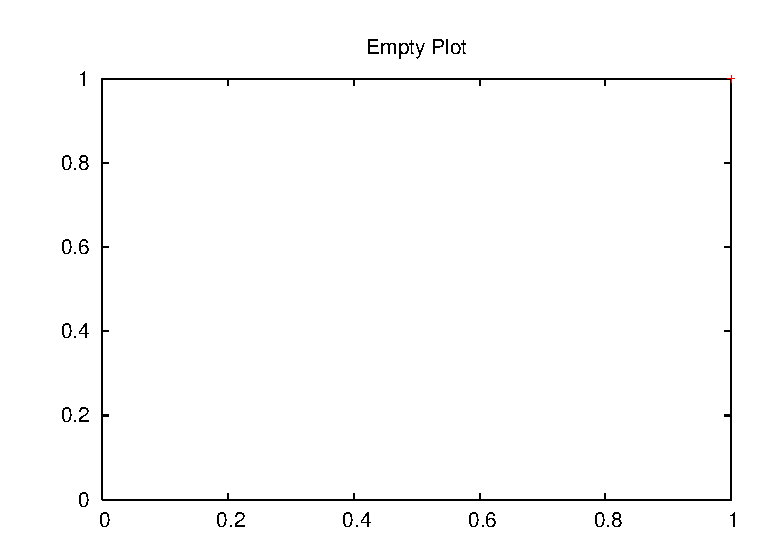
\includegraphics[height=1in]{F/empty.eps}
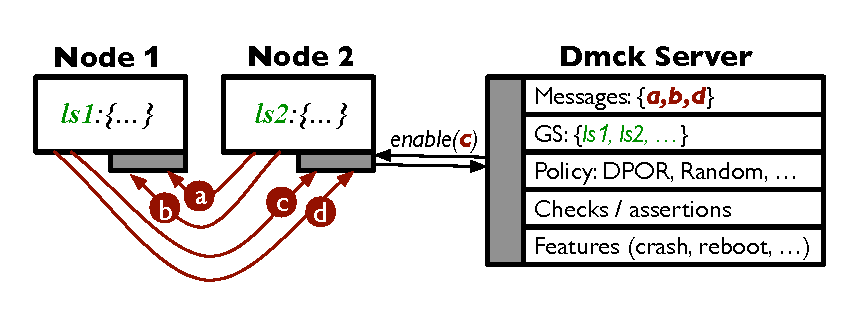
\includegraphics[height=2in]{F/dmck/dmck.eps}
}
\vminfive
\mycaption[Distributed System Model Checker]{fig-dmck}{DMCK}{The figure illustrates a typical framework
of a distributed system model checker (dmck).
}
%\vminten
\end{figure}

\if 0
The figure shows a dmck server model checking
a target distributed system containing two nodes.  
Communications in the target system are interposed 
\fi

 % -- pics

Although \modist's speed-up is significant, we find that one
scalability limitation of its DPOR application is within its {\em
  black-box} approach; it only exploits general properties of
distributed systems to define message independence.  It does not
exploit any semantic information from the target system to define more
independent events.  We will discuss this issue later
(\sec\ref{sam-ex}).








\begin{figure*}[t]

\centerline{
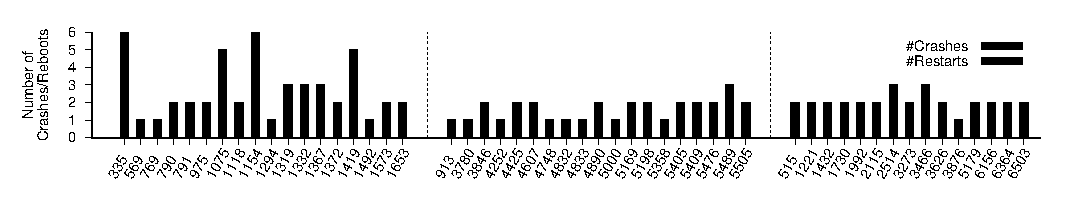
\includegraphics[width=6.5in]{F/deepbugs/eps/all.eps}
%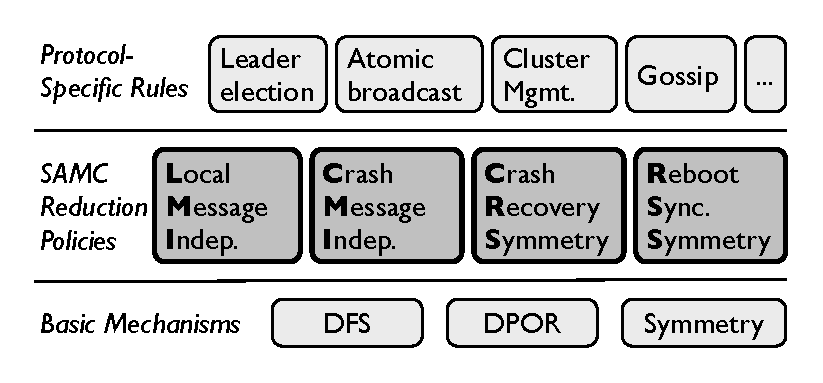
\includegraphics[height=1.2in]{F/samc/samc.eps}
}
\scriptsize{
~~~~~~~~~~~~~~~~~~~~~~~~~~~~~~~~~~~~~~\textsf{ZooKeeper Bugs}
~~~~~~~~~~~~~~~~~~~~~~~~~~~~~~~~~~~~\textsf{Hadoop MapReduce Bugs}
~~~~~~~~~~~~~~~~~~~~~~~~~~~~~~~\textsf{Cassandra Bugs}}
\vminfive
\mycaption[Deep Bugs]{fig-deepbugs}{Deep Bugs}{
%
The figure lists deep bugs from our bug study and depicts how many
crashes and reboots must happen to reproduce the bugs. Failure events
must happen in a specific order in a long sequence of events.  These
bugs came from many protocols including ZooKeeper leader election and
atomic broadcast, Hadoop MapReduce speculative execution, job/task
trackers, and resource/application managers, and Cassandra gossiper,
anti-entropy, mutation, and hinted handoff.  These bugs led to failed
jobs, node unavailability, data loss, inconsistency, and corruption.
They were labeled as ``major'', ``critical'', or ``blocker''.  12 of
these bugs happened within the last one year.  The median response
time (\ie, time to fix) is two weeks. There are few bugs that involve
4+ reboots and 4+ crashes that we do not show here.
%
} 
%\vminten

\end{figure*}

 % -- pics

% ------------------------------------------------------

% deemter
Dynamic interface reduction (DIR)~\cite{Guo+11-Demeter} is the next
advancement to \modist.  This work suggests that a complete dmck must
re-order not only messages (global events) but also thread
interleavings (local events).  The reduction intuition behind DIR is
that different thread interleavings often lead to the same global
events (\eg, a node sends the same messages regardless of how threads are
interleaved in that node).  DIR records local exploration and replays
future incoming messages without the need for global exploration.  
In our work, SAMC focuses only on global exploration (message and failure
re-orderings).  We believe DIR is orthogonal to SAMC, similar to the
way DIR is orthogonal to \modist.


% besides (quick take)
\modist\ and DIR are examples of dmcks that employ advanced systematic
reduction policies.  LMC~\cite{Guerraoui+11-McNoNetwork} is similar to
DIR; it also decouples local and global exploration.
dBug~\cite{Simsa+10-Dbug} applies DPOR similarly to \modist.  There are
other dmcks such as \macemc~\cite{Killian+07-LifeDeathMaceMC} and
CrystalBall~\cite{Yabandeh+09-CrystalBall} that use basic exploration
methods such as depth first (DFS), weight-based,
and random searches.

% symmetry
Other than the aforementioned methods, {\em symmetry} is another
foundational reduction policy~\cite{Emerson+97-PorAndSym,
  Prasad+00-SymBasedMc}.  Symmetry-based methods exploit the
architectural symmetry present in the target system.  For example, in
a ring of nodes, one can rotate the ring without affecting
the behavior of the system.  Symmetry is powerful, but 
we find no existing dmcks that adopt symmetry.

% multiple failures
Besides dmcks, there exists sophisticated testing frameworks for
distributed systems (\eg, \fate~\cite{Gunawi+11-FateDestini},
\prefail~\cite{Joshi+11-PreFail},
\setsudo~\cite{Joshi+13-SetsudoTesting}, OpenStack
fault-injector~\cite{Ju+13-FaultResOpenStack}). This set of work
emphasizes the importance of multiple failures, but their major
limitation is that they are not a dmck.  That is, they cannot
systematically control and permute non-deterministic choices such as
message and failure reorderings.







\section{Deep Bugs}
\label{mot-deep}


\if 0
\tl{response to reviewer E, regarding fix time for each bug, and
encounter dep bugs that developers don't think are worth fixing.
    COMMENT: We can show the time since an issue was reported until it was
    closed, but we do not think that it tells us important information.
    Longer fix time does not mean it is harder to fix, it might mean
    developers asked for more information (e.g. Log files) and reporters
    need some time to gather that or wait until bugs happen again.  For the
    bugs that developers do not think they are worth to fix, yes we have
    seen some. The example of these bugs could be the wrong state of
    systems that eventually be detected and fixed by some error handle
    code. This kind of bugs makes a few nodes down for few minutes (before
    alive again) that developers think it is not that bad.}
\fi


% 94
% 54 total

% bug study
To understand the unique reliability challenges faced by cloud
systems, we performed a study of reliability bugs of three popular
cloud systems: ZooKeeper~\cite{Hunt+10-ZooKeeperPaper}, Hadoop
MapReduce~\cite{Kumar+13-Yarn}, and
Cassandra~\cite{Lakshman+09-Cassandra}.  We scanned through thousands
of issues from their bug repositories.  We then tagged complex
reliability bugs that can only be caught by a dmck (\ie, bugs that can
occur only on specific orderings of events).  We found 94
dmck-catchable bugs.\footnote[1]{Since this is a manual effort, we
  might miss some bugs.  We also do not report ``simple'' bugs (\eg,
  error-code handling) that can be caught by unit tests.}  Our major
finding is that 50\% of them are deep bugs (require complex
re-ordering of not only messages but also crashes and reboots).



% results, and observations
Figure~\ref{fig-deepbugs} lists the deep bugs found from our bug
study.  Many of them were induced by multiple crashes and reboots.
Worse, to reproduce the bugs, crash and reboot events must happen in a
specific order within a long sequence of events (\eg, the example bug
in \sec\ref{sec-intro}).  Deep bugs lead to harmful consequences (\eg,
failed jobs, node unavailability, data loss, inconsistency,
corruption), but they are hard to find.  We observe that since there
is no dmck that helps in this regard, deep bugs are typically found in
deployment (via logs) or manually, then they get fixed in few
weeks, but afterwards as code changes continuously, new deep bugs
tend to surface again.
% , as confirmed by cloud developers~\cite{ClouderaPC}.





\section{Does State of the-Art Help?}
\label{mot-summ}

We now combine our observations in the two previous sections and
describe why state-of-the-art dmcks do not address present reliability
challenges of cloud systems.



% policies and bugs, random
First, {\em existing systematic reduction policies often cannot find
  bugs quickly}.  Experiences from previous dmck developments suggest
that significant savings from sound reduction policies do not always
imply high bug-finding effectiveness~\cite{Guo+11-Demeter,
  Yang+09-Modist}.  To cover deep states and find bugs, many dmcks
revert to non-systematic methods such as randomness or manual
checkpoints.  For example, \modist\ combines DPOR with random walk to
``jump'' faster to a different area of the state space (\sec4.5
of~\cite{Yang+09-Modist}).  DIR developers find new bugs by manually
setting ``interesting'' checkpoints so that future state explorations
happen from the checkpoints (\sec5.3 of~\cite{Guo+11-Demeter}).  In
our work, although we use different target systems, we are able to
reproduce the same experiences above (\sec\ref{eval-oldbugs}).



% multiple failures
Second, {\em existing dmcks do not scale with the inclusion of failure
  events}.  Given the first problem above, exercising multiple
failures will just exacerbate the state-space explosion problem.  Some
frameworks that can explore multiple failures such as
\macemc~\cite{Killian+07-LifeDeathMaceMC} only do so in a random way;
however, in our experience (\sec\ref{eval-oldbugs}), randomness many
times cannot find deep bugs quickly.  \modist\ also enabled only one
failure.  In reality, multiple failures is a big reliability threat,
and thus must be exercised.


We conclude that finding systematic (no random/checkpoint) policies
that can find deep bugs is still an open dmck research problem.  We
believe without semantic knowledge of the target system, dmck hits a
scalability wall (as also hinted by DIR authors; \sec8
of~\cite{Guo+11-Demeter}).  In addition, as crashes and reboots need
to be exercised, we believe recovery semantics must be incorporated into
reduction policies.  All of these observations led us to SAMC, which
we describe next.











\chapter{Semantic-Aware Model Checking}
\label{sec-samc}



% one paragraph about samc, 
\section{Overview}
Semantic-aware model checking (SAMC) is a white-box model checking
approach that takes semantic knowledge of how events (\eg, messages,
crashes, and reboots) are processed by the target system and
incorporates that information in reduction policies.  To show the
intuition behind SAMC, we first give an example of  a simple leader
election protocol. Then, we present SAMC architecture and our four
reduction policies.







% nothing here, see sam-overview









\section{An Example}
\label{sam-ex}

In a simple leader election protocol, every node broadcasts its vote to
reach a quorum and elect a leader.  Each node begins by voting for itself
(\eg, \ntwo\ broadcasts \ts{vote=2}).  Each node receives vote broadcasts
from other peers and processes every vote with this simplified code segment
below.  As depicted in the code segment below, if an incoming vote is less
than the node's current vote, it is simply discarded.  If it is larger, the
node changes its vote and broadcasts the new vote.

{\small
\begin{alltt}
  if (msg.vote < myVote) \{discard;\} 
  else \{myVote = msg.vote; broadcast(myVote);\}
\end{alltt}}



Let's assume \nfour\ with \ts{vote=4} is receiving three concurrent
messages with votes \ts{1}, \ts{2}, and \ts{3} from its peers.  Here,
a dmck with a black-box DPOR approach must perform 6 (3!) orderings
(\ts{123}, \ts{132}, and so on).  This is because a black-box DPOR
does {\em not} know the {\em message processing semantic} (\ie, how
messages will be processed by the receiving node).  Thus, a black-box
DPOR must treat all of them as dependent (\sec\ref{mot-state}); they
must be re-ordered for soundness.  However, by knowing the processing
logic above, a dmck can soundly conclude that all orderings will lead
to the same state; all messages will be discarded by \nfour\ and its local
state will not change.  Thus, a semantic-aware dmck can reduce the 6
redundant executions to just 1 execution.

The example above shows a scalability limitation of a black-box dmck.
Fortunately, simple semantic knowledge has a great potential in
removing redundant executions.  Furthermore, semantic knowledge can be
incorporated on top of sound model checking foundations such as DPOR
and symmetry, as we describe next.







\section{Architecture}
\label{sam-arch}





% figure, 3 mechanisms: abstractions (via history table), 
Figure~\ref{fig-samc} depicts the three levels of SAMC: sound
exploration mechanisms, reduction policies, and protocol-specific
rules.  SAMC is built on top of sound model checking foundations such
as DPOR~\cite{Flanagan+05-Dpor, Godefroid+96-Dpor} and
symmetry~\cite{Clarke+98-SymReduct, Prasad+00-SymBasedMc}.  We name
these foundations as mechanisms because a dmck must specify
accordingly what events are dependent/independent and symmetrical,
which in SAMC will be done by the reduction policies and
protocol-specific rules.






\begin{figure}[t]

\centerline{
%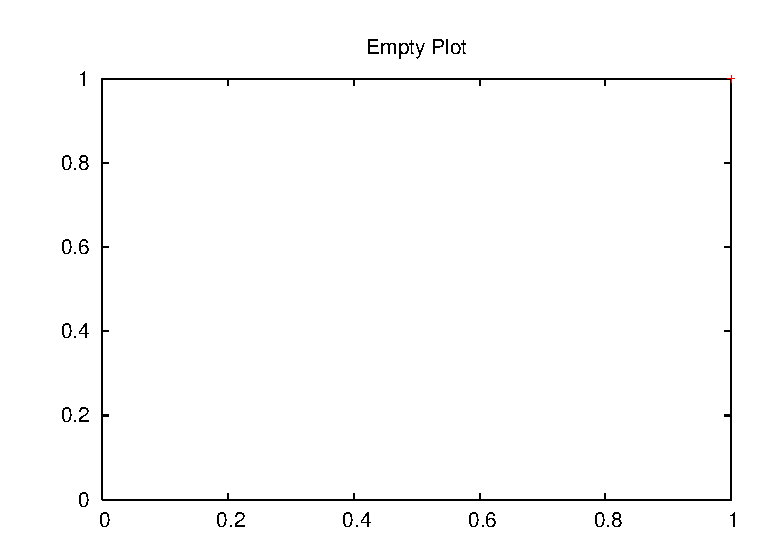
\includegraphics[height=1.4in]{F/empty.eps}
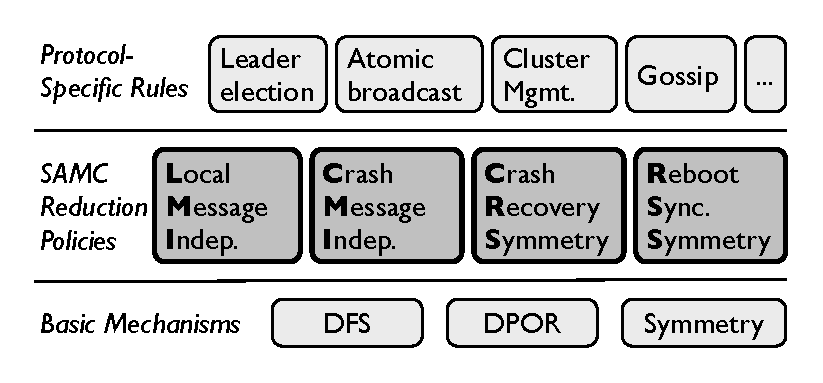
\includegraphics[height=2in]{F/samc/samc.eps}
}
\vminfive
\mycaption[SAMC Architecture]{fig-samc}{SAMC Architecture}{}
%\vminfive
\end{figure}

 % ------ fig samc

% 4 approaches and benefits
Our main contribution lies within our four novel {\em semantic-aware
  reduction policies}: local-message independence (LMI), crash-message
independence (CMI), crash recovery symmetry (CRS), and reboot
synchronization symmetry (RSS).  To the best of our knowledge, none of
these approaches have been introduced in the literature.  At the heart
of these policies are {\em generic event processing patterns} (\ie,
patterns of how messages, crashes, and reboots are processed by
distributed systems).  Our policies and patterns are simple and
powerful; they can be applied to many different distributed systems.  Testers
can extract the patterns from their target protocols (\eg,
leader election, atomic broadcast) and write protocol-specific
rules in few lines of code.

In the next section, we first present our four reduction policies
along with the processing patterns.  Later, we will discuss ways to
extract the patterns from target systems (\sec\ref{sam-extract}) and
then show the protocol-specific rules for our target systems
(\sec\ref{imp-targets}).





\section{Semantic-Aware Reduction Policies}
\label{sam-pol}



We now present four semantic-aware reduction policies that enable us to
define fine-grained event dependency/independency and symmetry beyond
what black-box approaches can do.




% policies




% ------------------------
\subsection{Local-Message Independence (LMI)}
\label{sam-lmi}





% LMI basic
We define {\em local messages} as messages that are concurrently in
flight to a given node (\ie, intra-node messages).  As shown in
Figure~\ref{fig-pol}a, a black-box DPOR treats the message processing
semantic inside the node as a black box, and thus must declare the
incoming messages as dependent, leading to 4! permutation
of \ma\mb\mc\md.  On the other hand, with white-box knowledge,
local-message independence (LMI) can define {\em independency
relationship among local messages}.  For example, illustratively in
Figure~\ref{fig-pol}b, given the node's local state (\ls) and the
processing semantic (embedded in the \ts{if} statement), LMI is able
to define that \ma\ and \mb\ are dependent, \mc\ and \md\ are
dependent, but the two groups are independent, which then leads to
only 4 re-orderings.  This reduction illustration is similar to the
one in Section~\ref{mot-state}, but this time LMI enables DPOR
application on local messages.


% LMI question
LMI can be easily added to a dmck.  A dmck server typically has a
complete view of the local states (\sec\ref{mot-bgterms}).  What is
needed is the {\em message processing semantic}: how will a node (\nn)
process an incoming message (\mm) given the node's current local state
(\ls)?  The answer lies in these four simple {\em message processing
patterns} (discard, increment, constant, and modify):


{\small
\begin{alltt}
     \underline{Discard:}           \underline{Increment:}  
     if (pd(m,ls))      if (pi(m,ls))
      (noop);             ls++;       

     \underline{Constant:}          \underline{Modify:}  
     if (pc(m,ls))      if (pm(m,ls))
       ls = Const;        ls = modify(m,ls);
\end{alltt}
}

% LMI pattern .....
In practice, \ls\ and \mm\ contain many fields.  For simplicity, we
treat them as integers.  The functions with prefix \pp\ are boolean
read-only functions (predicates) that compare an incoming message
(\mm) with respect to the local state (\ls); for example, \pd\ can
return true if \ts{m<s}.  The first pattern is a {\em discard} pattern
where the message is simply discarded if \pd\ is true.  This pattern
is prevalent in distributed systems with votes/versions; old
votes/versions tend to be discarded (\eg, our example
in \sec\ref{sam-ex}).  The {\em increment} pattern performs an
increment-by-one update if \pi\ is true, which is also quite common in
many protocols (\eg, counting commit acknowledgements).  The {\em
constant} pattern changes the local state to a constant whenever \pc\
is true.  Finally, the {\em modify} pattern changes the local state
whenever \pm\ is true.


% LMI policy
Based on these patterns, we can  apply LMI in the following
ways.
%
(1) \mx\ is independent of \my\ if \pd\ is true on any of \mx\ and \my.
That is, if \mx\ (or \my) will be discarded, 
then it does not need to be re-ordered 
with other messages.
%
(2) \mx\ is independent of \my\ if \pi\ (or \pc) is true on both \mx\ and \my.
That is, the re-orderings do not matter because the local state is
monotonically increasing by one (or changed to the same constant).
%
(3) \mx\ and \my\ are dependent if \pm\ is true on \mx\ and 
\pd\ is not true on \my.  
That is, since both messages modify the local state in unique ways, then the
re-orderings can be ``interesting'' and hence should be exercised.
%
All these rules are continuously evaluated before every event is
enabled.  If multiple cases are true, dependency has higher precedence
than independency.







% LMI, application 
Overall, LMI allows dmck to smartly skip redundant re-orderings by
leveraging simple patterns.  The job of the tester is to find the
message processing patterns from a target protocol and write {\em
protocol-specific rules} (\ie, filling in the content of the four LMI
predicate functions (\pd, \pi, \pc, and \pm) specific to the target
protocol).  As an example, for our simple leader election protocol
(\sec\ref{sam-ex}), \pd\ can be as simple as:
return \ts{m.vote} \ts{<}
\ts{ls.myVote}.









\begin{figure}[t]

\centerline{
%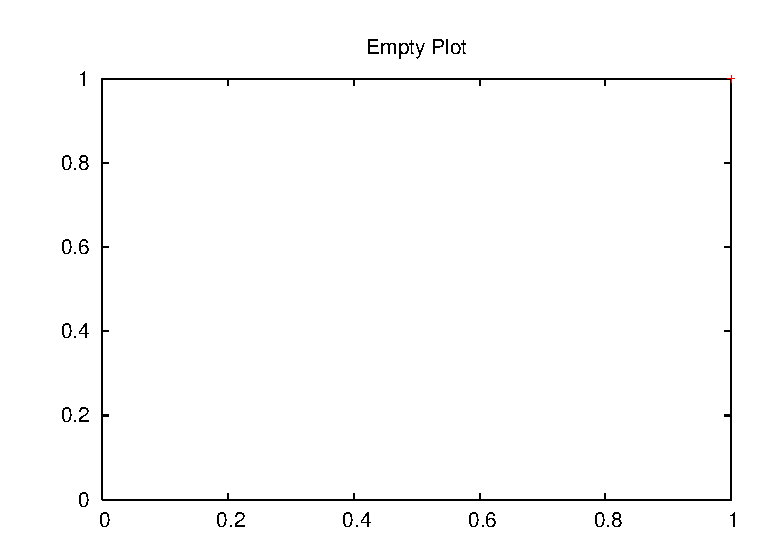
\includegraphics[height=1.2in]{F/empty.eps}
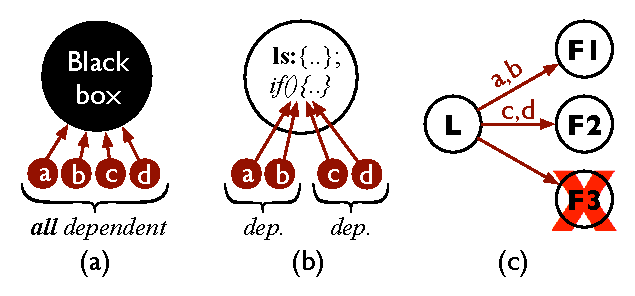
\includegraphics[height=2in]{F/pol/pol.eps}
}
\vminfive
\mycaption[LMI and CMI]{fig-pol}{LMI and CMI}{The figures
illustrate (a) a black-box approach, (b) local-message
independence with white-box knowledge, and (c)
crash-message independence.}
\vminten
\end{figure}





\subsection{Crash-Message Independence (CMI)}
\label{sam-cmi}


% CMI motivation
Figure~\ref{fig-pol}c illustrates the motivation behind our next
policy.  The figure resembles an atomic broadcast protocol where a
leader (\ts{L}) sends commit messages to the followers (\ts{F}s).
Let's assume commit messages \ts{ab} to \fone\ and \ts{cd} to \ftwo\
are still in flight (\ie, currently outstanding in the dmck; not
shown).  In addition, the dmck would like to crash \ftri, which we
label as a crash event \xx.  The question we raise is: how should \xx\
be re-ordered with respect to other outstanding messages
(\ma, \mb, \mc, and \md)?


% CMI problem dmck
As we mentioned before, we find {\em no} single dmck that incorporates
crash semantics into reduction policies.  As an implication, in our
example, the dmck must reorder \xx\ with respect to other outstanding
messages, generating executions \ts{Xabcd}, \ts{aXbcd}, \ts{abXcd},
and so on.  Worse, when \ts{abcd} are reordered, \xx\ will be
reordered again.  We find this as one major fundamental problem why
existing dmcks do not scale with the inclusion of failures.

% CMI pattern
To solve this, we introduce crash-message independence (CMI) which
defines {\em independency relationship between a to-be-injected crash
and outstanding messages}.  The key lies in these two crash reaction
patterns (global vs. local impact) running on the surviving nodes
(\eg, the leader node in Figure~\ref{fig-pol}c).


{\small
\begin{alltt}
      \underline{Global impact:}       \underline{Local impact:}
      if (pg(X,ls))         if (pl(X,ls)) 
        modify(ls);           modify(ls);
        sendMsg();           
\end{alltt}
}


% CMI pattern
The functions with prefix \pp\ are predicate functions that compare
the crash event \xx\ with respect to the surviving node's local state
(\eg, the leader's local state).  The \pg\ predicate in the {\em
global-impact} pattern defines that the crash \xx\ during the local
state \ls\ will lead to a local state change {\em and} new outgoing
messages (\eg, to other surviving nodes).  Here, no reduction can be
done because the new crash-induced outgoing messages must be
re-ordered with the current outstanding messages.  On the other hand,
reduction opportunities exist within the {\em local-impact} pattern,
wherein the \pl\ predicate specifies that the crash will just lead to
a local state change but not new messages, which implies that the
crash does not need to be re-ordered.  


% CMI policies
Based on the two crash impact patterns, we apply CMI in the following ways.
%
Given a local state \ls\ at node \nn, a peer failure \xx, and outstanding
messages (\mone...\mn) from \nn\ to other surviving peers, CMI performs:
%
(1) If \pl\ is true, then \xx\ and \mone...\mn\ are independent.
%
(2) If \pg\ is true, then \xx\ and \mone...\mn\ are dependent.
%
In Figure~\ref{fig-pol}c for example, if \pl\ is true in node \ts{L},
then \xx\ does not impact outstanding messages to \fone\ and \ftwo,
and thus \xx\ is independent to \ts{abcd}; exercising
\ts{Xabcd} is sufficient.


% CMI deployment
An example of CMI application is a quorum-based write protocol.  If a
follower crash occurs and quorum is still established, the leader will
just decrease the number of followers (local state change only).  Here,
for the protocol-specific rules, the tester can specify \pl\ with
\ts{\#follower} \ts{>=} \ts{majority} and \pg\ with the reverse. 
Overall, CMI helps dmck scale with the inclusion of failures, specifically by
skipping redundant re-orderings of crashes with respect to outstanding
messages.





% ---------------------------------
\subsection{Crash Recovery Symmetry (CRS)}
\label{sam-crs}


% RS Extra note
Before we discuss our next reduction policy, we emphasize again the
difference between message event and crash/reboot event.  Message
events are generated by the target system, and thus dmck can only
reduce the number of re-orderings (but it cannot reduce the events).
Contrary, crash events are generated by dmck, and thus there exists
opportunities to reduce the number of injected crashes.  For example,
in Figure~\ref{fig-pol}c, in addition to crashing \ftri, the dmck can
also crash \fone\ and \ftwo\ in different executions, but that might
not be necessary.

\input{code-crash}

% intuition: no individual node Ids, recovery depends on different states
To omit redundant crashes, we develop crash recovery symmetry (CRS).
The intuition is that some crashes often lead to symmetrical recovery
behaviors.  For example, let's assume a 4-node system with node
roles \ts{FFFL}.  At this state, crashing the first or second or third
node perhaps lead to the same recovery since all of them are
followers, and thereby injecting one follower crash could be enough.
Further on, if the system enters a slightly different
state, \ts{FFLF}, crashing any of the followers might give the same
result as above.  However, crashing the leader in the two cases
(\nfour\ in the first case and \ntri\ in the second) should perhaps be
treated differently because the recovery might involve the dead leader
ID.  The goal of CRS is to help dmck with crash decision.


% challenge
The main question in implementing CRS is: how to incorporate crash
recovery semantics into dmck?  Our solution is to compute {\em recovery
abstract global state} (\rags), a simple and concise representation of
crash recovery.  CRS builds \rags\ with the following steps:

First, we define that two recovery actions are symmetrical if they
produce the same messages and change the same local states in the same
way.

Second, we extract recovery logic from the code by flattening the
predicate-recovery pairs (\ie, recovery-related \ts{if} blocks).
Figure~\ref{code-crash} shows a simple example.  Different recovery
actions will be triggered based on which recovery predicate
(\prone, \prtwo, or \prtri) is true.  Each predicate depends on the
local state and the information about the crashing node.  Our key here
is to map each predicate-recovery pair to this formal pattern:


\vmintwo
{\small
\begin{alltt}
    if (\pri(ls, C.ls)) 
       modify(\ralsi); 
       \textit{(and/or)}
       sendMsg(\ralsi);
\end{alltt}
}
\vmintwo

Here, \pri\ is the recovery predicate for the i-th recovery action, and 
\ralsi\ is the recovery abstract local state 
(\ie, a subset of all fields of the local state involved in 
recovery).  That is, each recovery predicate defines what recovery
abstract local state that matters (\ie, \pri$\rightarrow$\{\ralsi\}).  For example, in Figure~\ref{code-crash},
if \prone\ is true, then \ralsone\ only contains the \ts{follower}
variable; if \prtri\ is true, \ralstri\ contains \ts{role}
and \ts{leaderId} variables.

Third, before we crash a node, we check which \pri\ will be true on
each surviving node and then obtain the \ralsi.  Next, we combine
\ralsi\ of all surviving nodes and {\em sort} them into a recovery
abstract global state (\rags);  sorting \rags\ helps us exploit
topological symmetry (\eg,  individual node IDs often do not matter).


Fourth, given a plan to crash a node, the algorithm above 
gives us the \rags\ that represents the corresponding recovery action.
We also maintain a history of \rags\ of previous injected crashes.
If the \rags\ already exists in the history, then the crash is skipped
because it will lead to a symmetrical recovery of the past.


% here here here
To recap with a concrete example, let's go back to the case
of \ts{FFFL} where we plan to enable crash(\none).  Based on the code
in Figure~\ref{code-crash}, the \rags\ is \{*, $\oslash$,
$\oslash$, \ts{\#follower=3}\}; 
* implies the crashing node, 
$\oslash$ means there is no true
predicate at the other two follower nodes, and \ts{\#follower=3} comes
from \ralsone\ of \prone\ of \nfour\ (the leader).  CRS will sort this
and check the history, and assuming no hit, then crash(\none) will be
enabled.  In another execution, SAMC finds that crash(\ntwo)
at \ts{FFFL} will lead to \rags:\{$\oslash$, *,
$\oslash$, \ts{\#follower=3}\}, which after sorting will hit the
history, and hence crash(\ntwo) is skipped.  If the system enters a
different state \ts{FFLF}, no follower crash will be injected, because
the \rags\ will be the same as above.  In terms of leader crash,
crashing the leader in the two cases will be treated differently
because in a leader crash, \prtri\ is true on followers and \prtri\
involves \ts{leaderId} which is different in the two cases.

% ...
In summary, the foundation of CRS is the computation of recovery
abstract global state (\rags) from the crash recovery logic extracted
from the target system via the \pri$\rightarrow$\{\ralsi\} pattern.
We believe this extraction method is simple because CRS does {\em not}
need to know the specifics of crash recovery; CRS just needs to know
what variables are involved in recovery (\ie, the \rals) .







\subsection{Reboot Synchronization Symmetry (RSS)}
\label{sam-rss}


Reboots are also essential to exercise (\sec\ref{mot-deep}), but if not
done carefully, will introduce more scalability problems.  Reboot reduction
policy is needed to help dmck inject reboots ``smartly''.  The intuition
behind reboot synchronization symmetry (RSS) is similar to that of CRS.
When a node reboots, it typically {\em synchronizes} itself with the peers.
However, a reboot will not lead to a new scenario if the current state of
the system is similar to the state when the node crashed.  To implement
RSS, we extract reboot-synchronization predicates and the corresponding
actions.  Since the overall approach is similar to CRS, we omit further
details.


In our experience RSS is extremely powerful.  For example, it allows
us to find deep bugs involving multiple reboots in the ZooKeeper
atomic broadcast (ZAB) protocol.  RSS works efficiently here because
reboots in ZAB are only interesting if the live nodes have seen new
commits (\ie, the dead node falls behind).  In contrast, a black-box
dmck without RSS initiates reboots even when the live nodes are in
similar states as in before the crash, prolonging the discovery of
deep bugs.





%\input{sam-ptop}
%\input{sam-pprio}




\section{Pattern Extraction}
\label{sam-extract}


% summary
We have presented four general, simple, and powerful semantic-aware
reduction policies along with the generic event processing patterns.
With this, testers can write protocol-specific rules by extracting the
patterns from their target systems.  
%
Given the patterns described in previous sections, a tester must
perform what we call as ``extraction'' phase.  Here, the tester must
extract the patterns from the target system and write
protocol-specific rules specifically by filling in the predicates and
abstractions as defined in previous sections; in
Section~\ref{imp-targets}, we will show a real extraction result (\ie,
real rules).  Currently, the extraction phase is manual; we leave
automated approaches as a future work (\sec\ref{discuss}).
Nevertheless, we believe manual extraction is bearable for several
reasons.  First, today is the era of
DevOps~\cite{Limoncelli+11-Devops} where developers are testers and
vice versa; testers know the internals of their target systems.  This
is also largely true in cloud system development.  Second, the
processing patterns only cover high-level semantics; testers just fill
in the predicates and abstractions but no more details.  In fact,
simple semantics are enough to significantly help dmck go faster to
deeper states.






\section{Summary}
In this chapter, we have introduced semantic-aware model checking or SAMC (pronounced
``Sam-C''). We have explained a basic concept and architecture, and explained
semantic-aware reduction policies in detail, including how to construct them by
extracting semantic knowledge from the code.











\chapter{Implementation and Integration}
\label{sec-impl}

\section{Overview}
In this chapter, we first describe our SAMC prototype, \sampro, which we
built from scratch because existing dmcks are either
proprietary~\cite{Yang+09-Modist} or only work on restricted high-level
languages (\eg, Mace~\cite{Killian+07-LifeDeathMaceMC}).  We will then describe
\sampro\ integration to three widely popular cloud systems,
ZooKeeper~\cite{Hunt+10-ZooKeeperPaper}, Hadoop/Yarn~\cite{Kumar+13-Yarn},
and Cassandra~\cite{Lakshman+09-Cassandra}.  Prior to \sampro, there was no
available dmck for these systems; they are still tested via unit tests, and
the test code size is bigger than the main code, but the tests are far from
reaching deep bugs.






\section{\sampro}
\label{imp-pro}

\sampro\ is written in \numLinesSamPro\ lines of code in Java, which
includes all the components mentioned in Section~\ref{mot-bgterms} and
Figure~\ref{fig-dmck}.  The detailed anatomy of dmck has been
thoroughly explained in literature~\cite{Guerraoui+11-McNoNetwork,
  Guo+11-Demeter, Killian+07-LifeDeathMaceMC, Simsa+10-Dbug,
  Yang+09-Modist}, and therefore for brevity, we will not discuss many
engineering details.  We will focus on SAMC-related parts.

% access source code
We design \sampro\ to be highly portable; we do not modify the target code
base significantly as we leverage a mature interposition technology,
AspectJ, for interposing network messages and timeouts.
% local state
Our interposition layer also sends local state information to the
\sampro\ server.
% crashes and reboots
\sampro\ is also equipped with crash and reboot scripts specific to the
target systems.  The tester can specify a budget of the maximum number of
crashes and reboots to inject per execution.
% summ
\sampro\ employs basic reduction mechanisms and advanced reduction policies
as described before.
% checks
We deploy safety checks at the server (\eg, no two leaders).  If a
check is violated, the trace that led to the bug is reported and 
can be deterministically replayed in \sampro.
% other supports
Overall, we have built all the necessary features to show the case of
SAMC.  Other features such as intra-node thread
interleavings~\cite{Guo+11-Demeter}, scale-out
parallelism~\cite{Simsa+12-ScalablePOR}, and virtual clock for network
delay~\cite{Yang+09-Modist} can be integrated to \sampro\ as well.




\vten % orphan text

\section{Integration to Target Systems}
\label{imp-targets}


In our work, the target systems are ZooKeeper, Hadoop 2.0/Yarn, and
Cassandra.  ZooKeeper~\cite{Hunt+10-ZooKeeperPaper} is a distributed
synchronization service acting as a backbone of many distributed systems
such as HBase and High-Availability HDFS.  Hadoop
2.0/Yarn~\cite{Kumar+13-Yarn} is the current generation of Hadoop that
separates cluster management and processing components.
Cassandra~\cite{Lakshman+09-Cassandra} is a distributed key-value store
derived from Amazon Dynamo~\cite{DeCandia+07-Dynamo}.

In total, we have model checked \numProtocols\ protocols: ZooKeeper
leader election (ZLE) and atomic broadcast (ZAB), Hadoop cluster
management (CM) and speculative execution (SE), and Cassandra
read/write (RW), hinted handoff (HH) and gossiper (GS).  These
protocols are highly asynchronous and thus susceptible to message
re-orderings and failures.

Table~\ref{tab-policies} shows a real sample of protocol-specific
rules that we wrote.  Rules are in general very short; we only wrote
\numLinesRule\ lines/protocol on average.  This shows the simplicity
of SAMC's integration to a wide variety of distributed system protocols.




\begin{sidewaystable*}
\begin{center}
{\small
%---------------------------------
\begin{tabular}{p{1.9in}|p{2in}|p{2.1in}|p{2in}} 


\multicolumn{1}{c|}{{\bf Local-Message}} &
\multicolumn{1}{c|}{{\bf Crash-Message}} &
\multicolumn{1}{c|}{{\bf Crash Recovery}} &
\multicolumn{1}{c}{{\bf Reboot Synchronization}}
\\

\multicolumn{1}{c|}{{\bf Independence (LMI)}} &
\multicolumn{1}{c|}{{\bf Independence (CMI)}} &
\multicolumn{1}{c|}{{\bf Symmetry (CRS)}} &
\multicolumn{1}{c}{{\bf Symmetry (RSS)}}
\\


\hline  % =====================================================

% ----------------------------------------------- ZLE, LMI (1)

\vminten
{\footnotesize
\begin{alltt}
bool pd : !newVote(m, s);

bool pm : newVote(m, s);

bool newVote(m, s) : {
 if (m.ep > s.ep) 
   return true; 
 else if (m.ep == s.ep)
  if (m.tx > s.tx) 
   return true;
  else if (m.tx == s.tx &&
           m.lid > s.lid) 
   return true;
}
\end{alltt}
}

& % ----------------------------------------------- ZLE, CMI (1)

\vminten
{\footnotesize
\begin{alltt}
bool pg (s, X) : 
 if (s.rl == F && X.rl == L)
  return true;
 if (s.rl == L && X.rl == F
     && !quorumAfterX(s)
  return true;
 if (s.rl == S && X.rl == S) 
  return true;

bool pl (s, X) :
 if (s.rl == L && X.rl == F 
     && quorumAfterX(s)) 
  return true;

bool quorumAfterX(s) :
  ret ((s.fol-1) >= 
        s.all/2);
\end{alltt}
}

& % ----------------------------------------------- ZLE, CRS (1)

\vminten
{\footnotesize
\begin{alltt}
bool pr1(s,C):
 if (s.rl == L && C.rl == F
     && quorumAfterX(s))
  return true;
rals1:\{rl,fol,all\};

bool pr2(s,C):
 if (s.rl == L && C.rl == F 
     && !quorumAfterX(s))
 return true;
rals2: \{rl,fol,lid,ep,tx,clk\}

bool pr3(s,C):
 if (s.rl == F && c.rl == L)
  return true;
rals3: \{rl,fol,lid,ep,tx,clk\}

bool pr4:
 if (s.rl == S)
  return true;
rals4: \{rl,lid,ep,tx,clk\}
\end{alltt}
}


& % ----------------------------------------------- ZLE, RSS (1)

\vminten
{\footnotesize
\begin{alltt}
bool ps1(s,R):
 if (s.rl == L)
  return true;
sals1: \{rl,lid,ep,tx,clk\}

bool ps2(s,R):
 if (s.rl == F)
  return true;
sals2: \{rl,lid,ep,tx,clk\}

bool ps3(s,R):
 if (s.rl == S && 
     s.clk > R.clk)
  return true;
sals3: \{rl,lid,ep,tx,clk\}

bool ps4(s,R):
 if (s.rl == S && 
     moreUpdated(s, R))
  return true;
sals4: \{rl,lid,ep,tx,clk\}

bool moreUpdated(s, R):
 if (R.ep > s.ep)
  return true;
 else if (R.ep == s.ep)
  if (R.tx > s.tx) 
   return true;
  else if (R.tx == s.tx)
   if (R.lid > s.lid)
    return true;
\end{alltt}
}

\end{tabular}
}
%---------------------------------
\end{center}
%
\vminfive
\mycaption[Protocol-Specific Reduction Rules for ZLE]{tab-policies}{Protocol-Specific Reduction Rules for ZLE}{
%
The code above shows the actual protocol-specific rules for
ZLE protocol.  These rules are the inputs to the four reduction policies.
%
Many variables are abbreviated (ep: epoch, tx: latest
transaction ID, lid: leader ID, rl: role, fol: follower count, all: total
node count, clk: logical clock, L: leading, F: following, S: searching,
X/C: crashing node, R: rebooting node). LMI \pc\ and \pi\ predicates are not 
used for ZLE, but used for other protocols. 
%
}
%\vminfive
\end{sidewaystable*}


\if 0
zle-specific rule = 49
zab-specific rule = 33
mapreduce: 35 ..
protocol average = 
\fi



\section{Summary}
In this chapter, we have talked about our prototype \sampro \; we have showed
technical detail how we built it and what cloud systems we targeted. In
addition, to give a sense of how protocol-specific reduction rules look like,
we have given an example of the rules for ZLE protocol.



\if 0
\input{imp-policy}
\input{imp-cases}

\fi







\chapter{Evaluation}
\label{sec-eval}


\section{Overview}
We now evaluate SAMC by presenting experimental results that answer the
following questions: 
\begin{enumerate}
\item How fast is SAMC in finding deep bugs compared to other state-of-the-art techniques?  
\item Can SAMC find new deep bugs?  
\item How much reduction ratio does SAMC provide?
\end{enumerate}

\if 0
(1) How fast is SAMC in finding deep bugs compared to
other state-of-the-art techniques?  (2) Can SAMC find new deep bugs?  (3)
How much reduction ratio does SAMC provide?
\fi

To answer the first question, we show SAMC's effectiveness in finding old
bugs.  For this, we have integrated \sampro\ to old versions of our target
systems that carry deep bugs: ZooKeeper v3.1.0, v3.3.2, v3.4.3, and v3.4.5,
Hadoop v2.0.3 and v2.2.0, and Cassandra v1.0.1 and v1.0.6.  To answer the
second question, we have integrated \sampro\ to two recent stable versions:
ZooKeeper v3.4.6 (released March 2014) and Hadoop v2.4.0 (released April
2014).  In total, we have integrated \sampro\ to \numVersions\ versions,
showing the high portability of our prototype.  Overall, our extensive
evaluation exercised more than 100,000 executions and used approximately 48
full machine days.




\if 0
\hsg{mention code coverage, and path coverage are hard
to quantify in Java code, or less priority}.
\fi







\section{Speed in Finding Old Bugs}
\label{eval-oldbugs}







\begin{figure}

% MR-5505: CM
\begin{center}
\fbox{
\begin{minipage}{5.5in}
{\bf \mr{5505}:}
\begin{enumerate}
\item A job finishes,
\item Application manager (AM) sends a ``remove-app'' message to Resource Manager (RM),
\item RM receives the message,
\item AM is unregistering,
\item \fev{RM crashes} before completely processes the message,
\item AM finishes unregistering,
\item \fev{RM reboots} and reads the old state file,
\item RM thinks the job has never started and runs the job again.
\end{enumerate}
%\ev{(1)} A job finishes,
%\ev{(2)} Application manager (AM) sends a ``remove-app'' message
%to Resource Manager (RM),
%\ev{(3)} RM receives the message,
%\ev{(4)} AM is unregistering,
%\ev{(5)} \fev{RM crashes} before completely processes the message,
%\ev{(6)} AM finishes unregistering,
%\ev{(7)} \fev{RM reboots} and reads the old state file,
%\ev{(8)} RM thinks the job has never started and runs the job again.
\end{minipage}
}
\end{center}


% CASS-3395: Hinted handoff
\vten
\begin{center}
\fbox{
\begin{minipage}{5.5in}
{\bf \cs{3395}}
\begin{enumerate}
\item Three nodes N1-3 started and formed a ring,
\item Client writes data,
\item \fev{N3 crashes},
\item Client updates the data via N1; N3 misses the update,
\item \fev{N3 reboots},
\item N1 begins the hinted handoff process,
\ev{(7)} Another client reads the data with strong consistency via N1 as
a coordinator,
\item N1 and N2 provide the updated value, but N3 still provides
the stale value,
\item The coordinator gets ``confused'' and returns the stale value to
the client!
\end{enumerate}
%\ev{(1)} Three nodes N1-3 started and formed a ring,
%\ev{(2)} Client writes data,
%\ev{(3)} \fev{N3 crashes},
%\ev{(4)} Client updates the data via N1; N3 misses the update,
%\ev{(5)} \fev{N3 reboots},
%\ev{(6)} N1 begins the hinted handoff process,
%\ev{(7)} Another client reads the data with strong consistency via N1 as
%a coordinator,
%\ev{(8)} N1 and N2 provide the updated value, but N3 still provides
%the stale value,
%\ev{(9)} The coordinator gets ``confused'' and returns the stale value to
%the client!
\end{minipage}
}

\end{center}


% MR 5863 (new)




\mycaption[Complexity of Deep Bugs]{code-oldbugs}{Complexity of Deep Bugs}{
%
Above are two sample deep bugs in Hadoop and Cassandra.  A sample
for ZooKeeper was shown in the introduction
(\sec\ref{sec-intro}).  Deep bugs are complex to reproduce; crash and
reboot events must happen in a specific order within a long sequence of
events (there are more events behind the events we show in the
bug descriptions above).
To see the high degree of complexity of other old bugs
that we reproduced, interested readers can click the
  issue numbers (hyperlinks) in Table~\ref{tab-oldbugs}.
%
}
%\vminfive
\end{figure}



\if 0

% CASS-3626: Gossiper
\vten
\fbox{
\begin{minipage}{2.95in}
{\bf \cassandra{3626}}
\ev{(1)} Three nodes N1, N2, and N3 start, sending join messages,
\ev{(2)} N1 receives message from N3,
\ev{(3)} N2 receives message from N3,
\ev{(4)} \fev{N3 crashes before} it detects its peers,
\ev{(5)} N1 receives message from N2,
\ev{(6)} N2 receives message from N1,
\ev{(7)} \fev{N2 crashes},
\ev{(8)} N1 detects N2 and N3 are down,
\ev{(9)} \fev{N3 reboots},
\ev{(10)} N3 wrongly believes N2 is up.
\end{minipage}
}
\fi



This section evaluates the speed of SAMC vs. state-of-the-art
techniques in finding old deep bugs.  In total, we have reproduced
\numOldDeepBugs\ old deep bugs (\numZkDeepBugs\ in ZooKeeper,
\numMrDeepBugs\ in Hadoop, and \numCsDeepBugs\ in Cassandra).
Figure~\ref{code-oldbugs} illustrates the complexity of the deep bugs
that we reproduced.



\def \fth {\uuu 5000}



\begin{table*}[!hbt]
\begin{center}
{\small
%---------------------------------
\begin{tabular}{l|l|ccc|rrrr|rrr} 

 {} & {} &
 {} & {} & {} &
\multicolumn{4}{c|}{{\bf \#Executions }} &
\multicolumn{3}{c}{{\bf Speed-up of SAMC vs. }} \\


{\bf Old Issue\#}  &  {\bf Protocol} & 
{\bf E} & {\bf C} & {\bf R} &
\bf{bDP} & \bf{RND} & \bf{rDP} & \bf{SAMC} &
\bf{bDP} & \bf{RND} & \bf{rDP} \\

\hline
\zk{335}   &   ZAB  & 120 & 3 & 3  &  \fth &  1057 &  \fth &   117 &  \uu 43 &      9 & \uu 43 \\
\zk{790}   &   ZLE  &  21 & 1 & 1  &    14 &   225 &    82 &     7 &       2 &     32 &     12 \\
\zk{975}   &   ZLE  &  21 & 1 & 1  &   967 &    71 &   163 &    53 &      18 &      1 &      3 \\
\zk{1075}  &   ZLE  &  25 & 3 & 2  &  1081 &    86 &   250 &    16 &      68 &      5 &     16 \\
\zk{1419}  &   ZLE  &  25 & 3 & 2  &   924 &  2514 &   987 &   100 &       9 &     25 &     10 \\
\zk{1492}  &   ZLE  &  31 & 1 & 0  &  \fth &  \fth &  \fth &   576 &   \uu 9 &  \uu 9 &  \uu 9 \\
\zk{1653}  &   ZAB  &  60 & 1 & 1  &   945 &  3756 &  3462 &    11 &     86  &    341 &    315 \\
\hline
\mr{4748}  &    SE  &  25 & 1 & 0  &    22 &     6 &     6 &     4 &       6 &      2 &      2 \\
\mr{5489}  &    CM  &  20 & 2 & 1  &  \fth &  \fth &  \fth &    53 &  \uu 94 & \uu 94 & \uu 94 \\
\mr{5505}  &    CM  &  40 & 1 & 1  &  1212 &  \fth &  1210 &    40 &      30 & \uu125 &     30 \\
\hline
\cs{3395}  & RW+HH  &  25 & 1 & 1  &  2552 &   191 &   550 &   104 &      25 &      2 &      5 \\
\cs{3626}  &    GS  &  15 & 2 & 1  &  \fth &  \fth &  \fth &    96 &  \uu 52 & \uu 52 & \uu 52 \\
\end{tabular}
}
%\vminten
%---------------------------------
\end{center}
\mycaption{tab-oldbugs}{SAMC Speed in Finding Old Bugs}{
%
``E'', ``C''
and ``R'' represent the number of events, crashes, and reboots
necessary to hit the bug.  The numbers in the middle four columns
represent the number of executions to hit the bug across different
policies.  ``bDP'', ``RND'', and ``rDP'' stand for black-box DPOR (in
\modist), random, and random + black-box DPOR respectively.
%Numbers marked with ``\nu'' imply that the experiments are still running
%at the time of this paper submission and the bug has not been reached.
We stop at 5000 executions (around 2 days) if the bug
cannot be found (labeled with ``\uuu'').  
Thus, speed-up numbers marked with
``\uu'' are potentially much higher.  
%
}

%\vminfive

\end{table*}

\if 0
\zk{1653}  &    --  & --- & 1 & 1  &    -- &    -- &    -- &    -- &     --- & --- & --- \\
\fi


Table~\ref{tab-oldbugs} shows the result of our comparison.  We
compare SAMC with basic techniques (DFS and Random) and advanced
state-of-the-art techniques such as black-box DPOR (``bDP'') and
Random+bDP (``rDP'').  Black-box DPOR is the \modist-style of DPOR
(\sec\ref{mot-state}).  We include Random+DPOR to mimic the way
\modist\ authors found bugs faster (\sec\ref{mot-summ}).  The table
shows the number of executions to hit the bug.  As a note,
software model checking with the inclusion of failures
takes time (back-and-forth communications between the target system
and the dmck server, killing and restarting system processes multiple
times, restarting the whole system from a clean state, \etc).  On
average, each execution runs for \numAvgExecTime\ seconds and involves
a long sequence of 20-120 events including the necessary crashes and
reboots to hit the bug.  We do not show the result of running DFS
because it never hits most of the bugs.  


Based on the result in Table~\ref{tab-oldbugs}, we make several
conclusions.
%
First, with SAMC, we prove that smart systematic approaches can reach
to deep bugs quickly.  We do not need to revert to randomness or
incorporate checkpoints.  As a note, we are able to reproduce every
deep bug that we picked; we did not skip any of them.
%
(Hunting more deep bugs is possible, if needed).

Second, SAMC is one to two orders of magnitude faster compared to
state-of-the-art techniques.  Our speed-up is up to
\numMaxBugSpeedUp\ (\numAvgBugSpeedUp\ on average).  But most
importantly, there are bugs that other techniques cannot find even
after 5000 executions (around 2 days). Here, SAMC's speed-up factor is
potentially much higher (labeled with ``\uu'').  Again, in the context of
dmck (a process of hours/days), large speed-ups matter.  In many
cases, state-of-the-art policies such as bDP and rDP cannot reach the
bugs even after very long executions.  The reasons are the two
problems we mentioned earlier (\sec\ref{mot-summ}).  Our
micro-analysis (not shown) confirmed our hypothesis that non-SAMC
policies frequently make redundant crash/reboot injections and event
re-orderings that anyway lead to insignificant state changes.

Third, Random is truly ``random''.  Although many previous dmcks
embrace randomness in finding bugs~\cite{Killian+07-LifeDeathMaceMC,
  Yang+09-Modist}, when it comes to failure-induced bugs, we have a
different experience.  Sometimes Random is as competitive as SAMC
(\eg, \zkb{975}), but sometimes Random is much slower (\eg,
\zkb{1419}), or worse Random sometimes did not hit the bug (\eg,
\zkb{1492}, \mrb{5505}).  We find that some bugs require crashes
and/or reboots to happen at very specific points, which is
probabilistically hard to reach with randomness.  With SAMC, we show
that being systematic and semantic aware is consistently effective.




\section{Ability of Finding New Bugs}
\label{eval-newbugs}

The previous section was our main focus of evaluation.  In addition to
this, we have integrated \sampro\ to recent stable versions of ZooKeeper
(v3.4.6, released March 2014) and Hadoop (v2.4.0, released April 2014).  In
just hours of deployment, we found \numZkNewBugs\ new ZLE bug involving 2
crashes, 2 reboots, and 52 events, and \numMrNewBugs\ new Hadoop
speculative execution bug involving 2 failures and 32 events.  These two
new bugs are distributed data race bugs.  The ZLE bug causes the ZooKeeper
cluster to create two leaders at the same time.  The Hadoop bug causes a
speculative attempt on a job that is wrongly moved to a scheduled state,
which then leads to an exception and a failed job.  We can
deterministically reproduce the bugs multiple times and we have reported
the bugs to the developers.  Currently, the bugs are still marked as major
and critical, the status is still open, and the resolution is still
unresolved.

\newtext{
We also note that in order to unearth more bugs, a dmck must have several
complete features: workload generators that cover many protocols,
sophisticated perturbations (\eg, message re-ordering, fault injections)
and detailed checks of specification violations.  Further discussions can
be found in our previous work~\cite{Gunawi+11-FateDestini}.  Currently,
\sampro\ focuses on speeding up the perturbation part.  By deploying more
workload generators and specification checks in \sampro, more deep bugs are
likely to be found.  As an illustration, the 94 deep bugs we mentioned in
Section~\ref{mot-deep} originated from various protocols and violated a wide
range of specifications.
}





\section{Reduction Ratio}
\label{eval-reduce}


Table~\ref{tab-reduce} compares the reduction ratio of SAMC over
black-box DPOR (bDP) with different budgets (\#crashes and \#reboots).
This evaluation is slightly different than the bug-finding speed evaluation
in Section~\ref{eval-oldbugs}.  Here, we measure how many executions in bDP
are considered redundant based on our reduction policies and
protocol-specific rules.  Specifically, we run bDP for
\numRedRatioExecs\ executions and run SAMC policies on the side to mark the
redundant executions.  The reduction ratio is then
\numRedRatioExecs\ divided by the number of non-redundant executions.
Table~\ref{tab-reduce} shows that SAMC provides between
\numMinRedRatio-\numMaxRedRatio\ execution reduction ratio in model
checking ZLE and ZAB protocols across different crash/reboot budgets.

\newtext{
Table~\ref{tab-reduce}b shows that with each policy the execution
reduction ratio increases when the number of crashes and reboots increases. 
With more crashes and reboots, the ZLE protocol generates more messages
and most of them are independent, and thus the LMI policy
has more opportunities to remove redundant message re-orderings.
Similary, the crash and reboot symmetry policies give better benefits
with more crashes and reboots.
The table also shows that LMI provides the most reduction.  This is because
the number of message events is higher than crash and reboot events
(as also depicted in Table~\ref{tab-oldbugs}).}

We now discuss our reduction ratio with that of DIR~\cite{Guo+11-Demeter}.
As discussed earlier (\sec\ref{mot-state}), DIR records local exploration
(thread interleavings) and replays future incoming messages whenever
possible, reducing the work of global exploration.  If the target system
does not have lots of thread interleavings, DIR's reduction ratio is
estimated to be between 10$^{1}$ to 10$^{3}$ (\sec5
of~\cite{Guo+11-Demeter}).  As we described earlier (\sec\ref{mot-state}),
DIR is orthogonal to SAMC.  Thus, the reduction ratios of SAMC and DIR are
complementary; when both methods are combined, there is a potential for a
higher reduction ratio.  The DIR authors also hinted that domain knowledge
can guide dmcks (and also help their work) to both scale and hit deep bugs
(\sec{8} of~\cite{Guo+11-Demeter}).  SAMC has successfully addressed such
need.





\begin{table}[t]
\begin{center}

{\small

\begin{tabular}{ll}
\begin{tabular}{cc|cc}
 & & \multicolumn{2}{c}{{\bf Execution Reduction Ratio in}} \\
{\bf C} & {\bf R} & {\bf ZLE} & {\bf ZAB} \\
\hline
%  0  &  0  &    19  &   750 \\
  1  &  1  &    37  &    93 \\
  2  &  2  &    63  &    107 \\
  3  &  3  &    103  &   166 \\
\end{tabular} &

%\vfifteen

\begin{tabular}{cc|ccccc}
 & & \multicolumn{5}{c}{{\bf \newtext{Execution Reduction Ratio in ZLE with}}} \\
{\bf C} & {\bf R} & {\bf All} & {\bf LMI} & {\bf CMI} & {\bf CRS} & {\bf RSS} \\
\hline
%  0  &  0  &    19  &   750 \\
  1  &  1  &    37  &   18  &   5  &   4  &   3  \\
  2  &  2  &    63  &   35  &   6  &   5  &   5  \\
  3  &  3  &    103 &   37  &   9  &   9  &   14  \\
\end{tabular} \\
 & \\
\multicolumn{1}{c}{(a)} & \multicolumn{1}{c}{(b)}
\end{tabular}

}
\end{center}
\vminten
\mycaption[SAMC Reduction Ratio]{tab-reduce}{SAMC Reduction Ratio}{
The table (a) shows the execution reduction ratio of SAMC
over black-box DPOR (bDP) in checking ZLE and ZAB
under different crash/reboot budgets.
``C'' and ``R'' are the number of crashes and reboots.
The table (b) shows the execution reduction ratio in ZLE
with individiual policies over black-box DPOR (bDP).
}
%\vminten
\end{table}




\if 0
method:
The way we compare the state space reduction is to run
DPOR, but on the side we keep track all other information, and if we find
the reorderings should be independent or symmetrical in SAMC, but bbDPOR
still does it, then we consider that as 1 saving.  Based on the total
number of savings, we compute the reduction ratio.
\fi



\if 0 


Just fill in the numbers here, and report me on skype everytime
you update every entry below.  Just copy paste the new updated entry.
On Skype.

SR: state reduction of SAMC / DPOR.

    C  R   SR
LE  0  0   19
LE  1  1   53 (3000) 64 (7000) 65 (6900)
LE  2  2   41 (3000) 57 (7000) 57 (7000)
LE  3  3   28 (3000) 35 (7000) 35 (7000)

ZAB  0  0   750 (1500ex) 
ZAB  1  1   35 (2000ex) 36 (1900)
ZAB  2  2   44 (2000ex) 44 (2000)
ZAB  3  3   142 (2000ex) 142 (2000)

\fi




\newtext{ Finally, we note that in evaluating SAMC, we use execution
  reduction ratio as a primary metric.  Another classical metric to
  evaluate a model checker is state coverage (\eg, a dmck that covers more
  states can be considered a more powerful dmck).  However, in our
  observation state coverage is not a proper metric for evaluating
  optimization heuristics such as SAMC policies.  For example, if there
  are three nodes ABC that have the same role (\eg, follower),  a naive
  black-box dmck will crash each node and covers three distinct states: *BC,
  A*C and AB*.  However, with a semantic-aware approach (\eg, symmetry), we
  know that covering one of the states is sufficient.  Thus, less state
  coverage does not necessarily imply a less powerful dmck.  }


\if 0
\tl{why we use reduction ratio instead of state coverage} We do not use
state coverage as our metric because we found that state coverage is not
equal to bug-finding effectiveness and this was also stated in
~\cite{Guo+11-Demeter}. For example, in our case, when we use CRS and RSS,
if we have three nodes and all of them are in the same state, CRS will try
killing only one node, but normal dmck will try to kill all of them. In
this case, SAMC covers only one state, but normal dmck covers three state,
however, SAMC is more effective to discover bugs rather than normal dmck
because it does not try redundant symmetrical execution. We can see from
this example that state coverage is not a good metric so we choose to use
reduction ratio of execution instead of state coverage.
\fi


% \input{eval-future}

\section{Summary}
In this chapter we have evaluated SAMC by anwering these three questions:
\begin{enumerate}
\item How fast is SAMC in finding deep bugs compared to other state-of-the-art techniques?  
\item Can SAMC find new deep bugs?  
\item How much reduction ratio does SAMC provide?
\end{enumerate}
Table~\ref{tab-oldbugs} answers the first question by showing that SAMC is one
to two orders of magnitude faster. And to answer the second question, we can
also show that SAMC can find new bugs in cloud systems by integrating it to the
newest vesion code. For the third question, we have answered it by
table~\ref{tab-reduce} showing reduction ratio of 37x - 166x compare to bDP.





\if 0
\input{eval-coverage}
\input{eval-scale}
\input{eval-error}

\input{eval-complex}

\input{eval-deepness}

\input{eval-related}
\fi







\chapter{Discussion}
\label{discuss}


% summary
\section{Overview}
In this section, we discuss SAMC's simplicity, generality and soundness.
We would like to emphasize that the main goal of this thesis is to show the
power of SAMC in finding deep bugs both quickly and systematically, and
thus we intentionally leave some subtasks (\eg, automated extraction,
soundness proofs) for future work.


% ---------------------------------
\section{Simplicity}

\newtext{In previous sections, we mentioned that policies can be written
  in few lines of code.  Besides LOC, simplicity can be measured by
  how much time  is required to understand a protocol
  implementation, extract the patterns and write the policies.  This time
  metric is unfortunately hard to quantify.  In our experience, the bulk of
  our time was spent in developing \sampro\ from scratch and
  integrating policies to dmck mechanisms (\sec\ref{mot-bgterms}).
  However, the process of understanding protocols and crafting policies
  requires a small effort (\eg, few days per protocol to the point where we
  feel the policies are robust).  We believe that the actual developers
  will be able to perform this process much faster than we did as they
  already have deeper understandings of their code.  }


% ---------------------------------
\section{Generality}
\label{sam-general}

Our policies contain patterns that are common in distributed systems.  One
natural question to ask is: how much semantic knowledge should we expose to
dmck?  The ideal case is to expose as much information as possible as long
as it is sound.  Since proving soundness and extracting patterns
automatically are our future work, in this thesis we only propose exposing
high-level processing semantics.  With advanced program analysis tools that
can analyze deep program logic, we believe more semantic knowledge can be
exposed to dmck in a sound manner.
%
\newtext{For example, LMI can be extended to include commutative
modifications.  This is possible if the program analysis can 
verify that the individual modification does not lead to other
state changes. }
%
This will perhaps be the point where symbolic execution and
dmck blend in the future (\sec\ref{sec-related}).


\newtext{
Nevertheless, we find that high-level semantics are powerful enough.
Beyond the three cloud systems we target in this thesis, 
we have been integrating SAMC to MaceMC~\cite{Killian+07-LifeDeathMaceMC}.
\macemc\ already employs random exploration policies to
model check Mace-based distributed systems such as Mace-based Chord and
Pastry.  
To integrate SAMC, we first must re-implement DPOR in MaceMC (existing
DPOR implementation in MaceMC is proprietary~\cite{Guo+11-Demeter}).
Then, we have written 18 lines of LMI protocol-specific rules for Chord
and attain two orders of magnitude of reduction in execution.
This shows the generality of SAMC to many distributed
systems.
}



% ---------------------------------
\section{Soundness}
\label{sam-sound}



\newtext{ 
%
SAMC policies only skip re-orderings and crash/reboot events that are
redundant by definition, however currently our version of SAMC is not
sound; the unsound phase is the manual extraction process.  For example, if
the tester writes a wrong predicate definition (\eg, \pd) that is
inconsistent with what the target system defines, then soundness (and
correctness) is broken.  Advanced program analysis tools can be developed
to automate and verify this extraction process and make SAMC sound.
Currently, the fact that protocol-specific rules tend to be short might
also help in reducing human errors.  Our prototype, \sampro, is no
different than other testing/verification tools; full correctness requires
that such tools to be free of bugs and complete in checking all specifications,
which can be hard to achieve.  Nevertheless, we want to bring up again the
discussion in Section~\ref{mot-summ} that dmck's scalability and ability to
find deep bugs in complex distributed systems are sometimes more important
than soundness.  We leave soundness proofs for future work, but we view
this as a small limitation, mainly because we have successfully shown the
power of SAMC.  }



\chapter{Related Work}
\label{sec-related}


\if 0
We now briefly discuss more related work on dmck and other approaches
to systems verification and testing.
\fi

\section{Existing Model Checkings}
% multiple failures
The threat of multiple failures to systems reliability already existed
since the P2P era; P2P systems are susceptible to ``churn'', the
continuous process of node joining and departing~\cite{Rhea+04-Churn}.
Many dmcks such as \macemc~\cite{Killian+07-LifeDeathMaceMC} and
CrystalBall~\cite{Yabandeh+09-CrystalBall} evaluate their approaches
on P2P systems.  Interestingly, we find that they mainly re-order join
messages.  To our understanding, based on their publications, they did
not inject and control node departures.  CrystalBall authors mentioned
about running churns, but only as part of their workloads, not as
events that the dmck can re-order.  This illustrates the non-triviality of
incorporating failures in dmck.

\section{Formal Model Checking Techniques}
% formal mc techniques .... 
Formal model checking foundations such as partial order
reduction~\cite{Flanagan+05-Dpor, Godefroid+96-Dpor},
symmetry~\cite{Clarke+98-SymReduct, Prasad+00-SymBasedMc}, and
abstraction~\cite{Clarke+94-McAbstract}, were established more than a
decade ago.  Here, classical model checkers require system models and
mainly focus on state-space reduction.  Implementation-level model
checkers on the other hand are expected to find real bugs in addition to
being efficient.

\section{Symbolic Execution}
% symbolic execution ...
Symbolic execution is another powerful formal method to verify
systems correctness.  Symbolic execution also faces an explosion
problem, specifically the path explosion problem.  A huge body of work
has successfully addressed the problem and made symbolic execution
scale to large (non-distributed) software
systems~\cite{Bucur+11-ParallelSymEx, Cadar+08-KLEE, Chipounov+11-S2e,
  Cui+13-RuleDirectedSymExec, Zamfir+10-Synthesis}.  Symbolic
execution and model checking can formally be combined into a more
powerful method~\cite{Burch+92-SymbolicMC}, however this concept has
not permeated the world of distributed systems; it is challenging to
track symbolic values across distributed nodes.


\section{Fault Injector}
% fault injector
Reliability bugs are often caused by incorrect handling of
failures~\cite{Gunawi+11-FateDestini, Gunawi+08-EIO}.  Fault-injection
testing however is challenging due to the large number of possible
failures to inject.  This challenge led to the development of
efficient fault-injection testing frameworks.  For example,
AFEX~\cite{Banabic+12-Blackbox} and
LFI~\cite{Marinescu+10-ExtensibleLFI} automatically prioritize
``high-impact targets'' (\eg, unchecked system calls).  These novel
frameworks target non-distributed systems and thus the techniques are
different than ours.


% distributed systems
Similarly, recent work highlights the importance of testing faults in
cloud systems (\eg, \fate~\cite{Gunawi+11-FateDestini},
\setsudo~\cite{Joshi+13-SetsudoTesting},
\prefail~\cite{Joshi+11-PreFail}, and OpenStack
fault-injector~\cite{Ju+13-FaultResOpenStack}).  As mentioned before
(\sec\ref{mot-state}), these frameworks are not a dmck; they cannot
re-order concurrent messages and failures and therefore cannot catch
distributed concurrency bugs systematically.



\section{Concurrency Bugs}
% local concurrency: Jula+08-DeadlockImmunity, Zhang+13-ConAir,
% Erickson+10-DataRaceKernel
The deep bugs we presented can be considered as concurrency bugs (in
distributed nature).  For non-distributed systems, there has been an
abundance of innovations in detecting, avoiding, and recovering from
concurrency bugs~\cite{Jin+12-CFix,
  Kasikci+13-CrowdRaceMob, 
  Lu+08-ConcurrencyBugStudy, 
  Veeraraghavan+11-ComplementarySchedules}.
They mainly target threads.  For dmck, we believe more advancements
are needed to unearth distributed concurrency bugs that still linger
in cloud systems.

\section{Geographically Distributed Systems}
% geo
\newtext{ Finally, the journey in increasing cloud dependability 
  is ongoing;  cloud systems face other issues such as bad error handling
  code~\cite{Yuan+14-Simplex}, performance failures~\cite{Do+13-Limplock},
  corruptions~\cite{Do+13-HARDFS}, and many others.  }
%
Exacerbating the
  problem, cloud systems are becoming larger and geographically
  distributed~\cite{Lloyd+11-Cops, Terry+13-PileusConsistencySLA,
    Zhang+13-TransactionChains}.  We believe cloud systems will observe
  more failures and message re-orderings, and therefore our work and future
  dmck advancements with the inclusion of failures will play an important
  role in increasing the reliability of future cloud systems.



\chapter{Conclusion and Future Work}
\section{Conclusion}
\label{sec-conclude}

Complex failures is a norm in cloud systems and deep bugs still linger in the
cloud.  To address present reliability challenges, dmcks must incorporate
complex failures, but due to the problem of state space explosion, existing
dmcks do not scale in this regard.  We strongly believe that without semantic
knowledge dmck hits a scalability wall.

In this thesis, we propose semantic-aware model checking (SAMC), a white-box
model checking approach that takes semantic knowledge and incorporates it in
reduction policies. 

We show a strong case that the SAMC principle can elegantly address this
scalability problem.  SAMC is simple and powerful; with simple semantic
knowledge, we show that dmcks can scale significantly.  We presented four
specific reduction policies, but beyond this, we believe our work triggers the
discussion of two important research questions: 
\begin{enumerate}
\item {\em What} other semantic knowledge can scale dmck?
\item {\em How} to extract white-box information from the target system? 
\end{enumerate}
We hope (and believe) that the SAMC principle can trigger future research in this
space.  



\section{Future}

\XXX{4 mins}

Well, that's all for my previous work. Now, I'll talk about my future work.

\subsection{Future Direction}

Here is my future direction

Toward DC bugs, TaxDC shows model checker needs to capture more events.

But to do that more challenges lie ahead, which I'll show.

For scalability bugs, they can happen in many axes, I just address one axe of
them. Many issues haven't been touched yet. I'll show you what are waiting for
us.

\subsection{DMCK}

Right now, SAMC doesn't address local computation timing, And also failure
model SAMC uses is only node fail-stop and reboot.

My first next step is advancing SAMC to capture local computation and expand
failure model.

The challenge here is this creates more events to re-order, and exacerbates
state space explostion.

So I will create more generic reduction policies to mitigate state space
explosion.

%In combating DC bugs, SAMC, a semantic aware model checker, leverage a domain
%specific knowledge to tackle state space explosion. 
%
%Right now, the generic patterns I exploit to build protocol-specific reduction
%policies are very simple. But this just scratches the surface of the power of
%semantic awareness. There are much more patterns and more reduction priciples
%waiting us to explore.
%
%So the next step on unearthing DC bugs is finding more patterns and creating
%more generic reduction policies, which will accelerate checking time.

%\subsection{AMC}

However, if you consider the current patterns I have here, they are very easy
to extract from the codebase.

Right now, we will have more reduction.

More reduction will find bugs faster, but that means extracting semantic
knowledge will be more complicated and harder.

This creates more burden on developers, and also introduce a chance of human
error.

And the error could leave bugs undetected..

My second step here will get rid of the burden of writing protocol-specific
policies by adopting program analysis to auto generate the policies.

%This will reduce the burden from developers and also the error.

\subsection{Scalability bugs}

Then let's look at scalability bugs. This class of bugs is new generation bugs
to combat in cloud-scale distributed systems.  And not much attention paid on
them. 

My vision here is to raise awareness on combating them.

On September this year, Cassandra developers started a new initiative to build
``Gossip 2.0'', by aiming at 1000 node cluster.

If they don't have a good way to test scalability, latent scalability bugs will
linger there. We might see a call for gossip 3.0 in a next few years.

%\subsection{4 axes}

As I said SCk is one of pilot works. It addresses only one axe of scalability,
which is scale of cluster.

From our cloud bug study, there are also

Scale of data

Scale of workload

And scale of failure

%SCk covers some part of scale of cluster. 

Previous work like Exalt covers some of scale of data. 

Many challenges lie ahead. In my future work, I'll adopt other techniques such
program analysis, to combat unsolved problems.



%\section{Conclusion}
\label{sec-conclude}

Complex failures is a norm in cloud systems and deep bugs still linger in the
cloud.  To address present reliability challenges, dmcks must incorporate
complex failures, but due to the problem of state space explosion, existing
dmcks do not scale in this regard.  We strongly believe that without semantic
knowledge dmck hits a scalability wall.

In this thesis, we propose semantic-aware model checking (SAMC), a white-box
model checking approach that takes semantic knowledge and incorporates it in
reduction policies. 

We show a strong case that the SAMC principle can elegantly address this
scalability problem.  SAMC is simple and powerful; with simple semantic
knowledge, we show that dmcks can scale significantly.  We presented four
specific reduction policies, but beyond this, we believe our work triggers the
discussion of two important research questions: 
\begin{enumerate}
\item {\em What} other semantic knowledge can scale dmck?
\item {\em How} to extract white-box information from the target system? 
\end{enumerate}
We hope (and believe) that the SAMC principle can trigger future research in this
space.  


%
\section{Future}

\XXX{4 mins}

Well, that's all for my previous work. Now, I'll talk about my future work.

\subsection{Future Direction}

Here is my future direction

Toward DC bugs, TaxDC shows model checker needs to capture more events.

But to do that more challenges lie ahead, which I'll show.

For scalability bugs, they can happen in many axes, I just address one axe of
them. Many issues haven't been touched yet. I'll show you what are waiting for
us.

\subsection{DMCK}

Right now, SAMC doesn't address local computation timing, And also failure
model SAMC uses is only node fail-stop and reboot.

My first next step is advancing SAMC to capture local computation and expand
failure model.

The challenge here is this creates more events to re-order, and exacerbates
state space explostion.

So I will create more generic reduction policies to mitigate state space
explosion.

%In combating DC bugs, SAMC, a semantic aware model checker, leverage a domain
%specific knowledge to tackle state space explosion. 
%
%Right now, the generic patterns I exploit to build protocol-specific reduction
%policies are very simple. But this just scratches the surface of the power of
%semantic awareness. There are much more patterns and more reduction priciples
%waiting us to explore.
%
%So the next step on unearthing DC bugs is finding more patterns and creating
%more generic reduction policies, which will accelerate checking time.

%\subsection{AMC}

However, if you consider the current patterns I have here, they are very easy
to extract from the codebase.

Right now, we will have more reduction.

More reduction will find bugs faster, but that means extracting semantic
knowledge will be more complicated and harder.

This creates more burden on developers, and also introduce a chance of human
error.

And the error could leave bugs undetected..

My second step here will get rid of the burden of writing protocol-specific
policies by adopting program analysis to auto generate the policies.

%This will reduce the burden from developers and also the error.

\subsection{Scalability bugs}

Then let's look at scalability bugs. This class of bugs is new generation bugs
to combat in cloud-scale distributed systems.  And not much attention paid on
them. 

My vision here is to raise awareness on combating them.

On September this year, Cassandra developers started a new initiative to build
``Gossip 2.0'', by aiming at 1000 node cluster.

If they don't have a good way to test scalability, latent scalability bugs will
linger there. We might see a call for gossip 3.0 in a next few years.

%\subsection{4 axes}

As I said SCk is one of pilot works. It addresses only one axe of scalability,
which is scale of cluster.

From our cloud bug study, there are also

Scale of data

Scale of workload

And scale of failure

%SCk covers some part of scale of cluster. 

Previous work like Exalt covers some of scale of data. 

Many challenges lie ahead. In my future work, I'll adopt other techniques such
program analysis, to combat unsolved problems.



% Format a LaTeX bibliography
\makebibliography

% Figures and tables, if you decide to leave them to the end
%\input{figure}
%\input{table}

\end{document}


